%%%%%%%%%%%%%%%%%%%%%%%%%%%%%%%%%%%%%%%%%%%%%%%%%%%%%%%%%%%%%%%%%%%%%%
% Lớp 12 | Phương trình mặt phẳng, đường thẳng, mặt cầu | Phương trình mặt cầu trong không gian
% Dạng 2H5?3-3: Viết phương trình tổng quát mặt cầu
% Số câu: 116  (sinh tự động bởi tach_cau.py; từ nay thầy sửa trực tiếp file này)
%%%%%%%%%%%%%%%%%%%%%%%%%%%%%%%%%%%%%%%%%%%%%%%%%%%%%%%%%%%%%%%%%%%%%%

%%%%%%%%%%%%%%%% TRẮC NGHIỆM 4 PHƯƠNG ÁN %%%%%%%%%%%%%%%%

% nguồn: Phan1_Lop_12_Hinh_hoc_Chuong_5
\begin{ex}%[2H5N3-3]%[ma:fd217718]
	Trong không gian $Oxyz$, cho mặt cầu $(S)$ có tâm  $I(1;2;-1)$ và bán kính bằng $2$. Phương trình mặt cầu $(S)$ là
	 \choice
		{$(x+1)^2+(y+2)^2+(z-1)^2=4$} 
		 {$(x-1)^2+(y-2)^2+(z+1)^2=2$}
		{\True $(x-1)^2+(y-2)^2+(z+1)^2=4$} 
		{$(x+1)^2+(y+2)^2+(z-1)^2=2$} 
	\loigiai{ 
		Mặt cầu $(S)$ có tâm $I(1;2;-1)$ và bán kính bằng $2$ nên phương trình mặt cầu $(S)$ là $(S)\colon (x-1)^2+(y-2)^2+(z+1)^2=4$. 
	} 
\end{ex}

% nguồn: Phan1_Lop_12_Hinh_hoc_Chuong_5
\begin{ex}%[2H5N3-3]%[ma:5c595067]
	Trong  không gian với hệ tọa độ $Oxyz$, trong các phương trình sau phương trình nào là phương trình của mặt cầu?
	 \choice
		 {\True $2x^2+2y^2+2z^2+4x+8y=0$}
		{$x^2+2y^2+z^2-2x+4y-2z-1=0$} 
		 {$x^2+y^2+z^2-2x+2y+3=0$}
		{$x^2+y^2-z^2-2x+2y-4z+8=0$} 
	 \loigiai{
		Phương trình $2x^2+2y^2+2z^2+4x+8y=0 \Leftrightarrow  x^2+y^2+z^2+2x+4y=0$.\\
		Có $a=-1$, $b=-4$, $c=0$, $d=0$ $\Rightarrow a^2+b^2+c^2-d>0$ nên  đó là phương trình mặt cầu.
	 }
\end{ex}

% nguồn: Phan1_Lop_12_Hinh_hoc_Chuong_5
\begin{ex}%[2H5N3-3]%[ma:409c7b0a]
	Trong không gian với hệ tọa  độ $Oxyz$, trong các phương trình sau phương trình nào là phương trình của mặt cầu?
	\choice 
		{\True  $x^2+y^2+z^2-2x+4z-1=0$}
		{$x^2+z^2+3x-2y+4z-1=0$} 
		{$x^2+y^2+z^2+2xy-4y+4z-1=0$} 
		 {$x^2+y^2+z^2-2x+2y-4z+8=0$}
	\loigiai{ 
		Phương trình $x^2+y^2+z^2-2ax-2by-2cz+d=0$ $(a^2+b^2+c^2-d>0)$ là  phương trình mặt cầu có tâm $I(a;b;c)$, bán kính $R=\sqrt{a^2+b^2+c^2-d}$.
		Phương  trình $x^2+y^2+z^2-2x+4z-1=0$ là phương trình mặt cầu vì $a^2+b^2+c^2-d=1+0+4+1=6>0$.
	} 
\end{ex}

% nguồn: Phan1_Lop_12_Hinh_hoc_Chuong_5
\begin{ex}%[2H5N3-3]%[ma:d64a688d]
	 Trong không gian với hệ trục tọa độ $Oxyz$, phương trình nào sau đây là phương trình mặt cầu?
	 \choice
		{$x^2 + y^2 + z^2 - 4x - 2y + 5  = 0$}
		{\True $x^2 + y^2 + z^2  - 4x + 1 = 0$}
		{$x^2 + y^2 + z^2 + 2x + 6y  - 2z + 15 = 0$}
		{$x^2  + y^2 + z^2 - 6z + 20 = 0$}
	 \loigiai{
		Phương  trình dạng $x^2+y^2+z^2-2ax-2by-2cx+d=0$ là phương trình mặt cầu khi và chỉ khi $a^2+b^2+c^2-d>0$.\\
		Xét phương trình $x^2 + y^2 + z^2 -  4x + 1 = 0$ có $a=2$, $b=0$, $c=0$, $d=1$.\\
		Vì $a^2+b^2+c^2-d=4+0+0-1=3>0$ nên phương trình trên  là phương trình mặt cầu.
	} 
\end{ex}

% nguồn: Phan1_Lop_12_Hinh_hoc_Chuong_5
\begin{ex}%[2H5N3-3]%[ma:a79f4afa]
	Trong không gian $Oxyz$, cho điểm $I(0;-3;1)$ và $R=2$. Mặt cầu tâm  $I$, bán kính $R$ có phương trình~là
	 \choice
		{\True  $x^2 +(y+3)^2 +(z-1)^2=4$}
		{$x^2 +(y-3)^2 +(z+1)^2=4$} 
		{$x^2  +(y+3)^2 +(z-1)^2=2$}
		{$x^2  +(y-3)^2 +(z+1)^2=2$}
	 \loigiai{
		Mặt cầu tâm $I(0;-3;1)$,  bán kính $R=2$ có phương trình~là
		$$x^2  +(y+3)^2 +(z-1)^2=4.$$
	} 
\end{ex}

% nguồn: Phan1_Lop_12_Hinh_hoc_Chuong_5
\begin{ex}%[2H5N3-3]%[ma:c730b73e]
	Trong không gian $Oxyz$, mặt cầu $(S)$ có  tâm là gốc tọa độ và bán kính $\sqrt{2}$ có phương trình là
	 \choice
		{\True $x^{2}+y^{2}+z^{2}=2$} 
		 {$(x-1)^{2}+y^{2}+z^{2}=1$}
		 {$x^{2}+y^{2}+z^{2}=\sqrt{2}$}
		 {$(x-1)^{2}+y^{2}+z^{2}=2$}
	 \loigiai{
	Mặt cầu $(S)$ có tâm  là gốc tọa độ và bán kính $\sqrt{2}$ có phương trình là $x^{2}+y^{2}+z^{2}=2$.}
\end{ex}

% nguồn: Phan1_Lop_12_Hinh_hoc_Chuong_5
\begin{ex}%[2H5N3-3]%[ma:def1e653]
	Trong không gian với hệ tọa độ $Oxyz$, trong các phương trình sau phương trình nào  không phải là phương trình của mặt cầu?
	\choice 
		{\True $x^2+2y^2+2z^2-2x+4z-1=0$} 
		{$x^2+y^2+z^2+3x-2y+4z-1=0$} 
		 {$x^2+y^2+z^2+2x-4y+4z-1=0$}
		{$x^2+y^2+z^2-2x+2y-4z-8=0$} 
	\loigiai{ 
		 Phương trình $x^2+2y^2+2z^2-2x+4z-1=0$ có hệ số trước $x^2$, $y^2$, $z^2$ không bằng nhau nên không phải là phương trình mặt cầu.
	 }
\end{ex}

% nguồn: Phan1_Lop_12_Hinh_hoc_Chuong_5
\begin{ex}%[2H5N3-3]%[ma:02c75e4b]
	Trong không gian $ Oxyz$, phương trình mặt cầu tâm $I\left(a;b;c\right)$ bán  kính $R$~là
	\choice 
		 {$(x-a)^2+(y-b)^2+(z+c)^2=R^2$}
		 {$(x-a)^2+(y+b)^2+(z-c)^2=R^2$}
		 {$(x+a)^2+(y+b)^2+(z+c)^2=R^2$}
		{\True  $(x-a)^2+(y-b)^2+(z-c)^2=R^2$}
	\loigiai{ 
		Phương trình mặt cầu tâm ${I}\left(a;b;c\right)$  bán kính $R$~là $(x-a)^2+(y-b)^2+(z-c)^2=R^2$.
	 }
\end{ex}

% nguồn: Phan1_Lop_12_Hinh_hoc_Chuong_5
\begin{ex}%[2H5N3-3]%[ma:69c208c8]
	Trong không gian $Oxyz$, mặt  cầu có tâm $I\left(2;1;-3\right)$ và bán kính $9$ có phương trình là
	\choice 
		 {\True $\left(x-2\right)^2+\left(y-1\right)^2+\left(z+3\right)^2=81$}
		{$\left(x+2\right)^2+\left(y+1\right)^2+\left(z-3\right)^2=81$} 
		{$\left(x-2\right)^2+\left(y-1\right)^2+\left(z+3\right)^2=9$} 
		{$\left(x+2\right)^2+\left(y+1\right)^2+\left(z-3\right)^2=9$} 
	\loigiai{ 
		Phương trình mặt cầu có tâm $I\left(2;1;-3\right)$ và bán kính $9$ là 
		\begin{align*}
			 \left(x-2\right)^2+\left(y-1\right)^2+\left(z+3\right)^2=81.
		\end{align*}
	} 
\end{ex}

% nguồn: Phan1_Lop_12_Hinh_hoc_Chuong_5
\begin{ex}%[2H5N3-3]%[ma:6c8ebee2]
	Trong không gian $Oxyz$, mặt cầu tâm $I(-7;8;9)$ đi  qua $A(-5;6;10)$ có phương trình~là
	\choice 
		{\True  $(x+7)^2+(y-8)^2+(z-9)^2=9$}
		 {$(x+7)^2+(y-8)^2+(z-9)^2=81$}
		{$(x+7)^2+(y-8)^2+(z-9)^2=3$} 
		 {$(x-7)^2+(y+8)^2+(z+9)^2=9$}
	\loigiai{ 
	Mặt cầu tâm $I(-7;8;9)$ đi qua $A(-5;6;10)$ có  phương trình~là
	$$(x+7)^2+(y-8)^2+(z-9)^2=9.$$ 
	 }
\end{ex}

% nguồn: Phan1_Lop_12_Hinh_hoc_Chuong_5
\begin{ex}%[2H5N3-3]%[ma:00af6eba]
	 Trong không gian với hệ tọa độ $Oxyz$, hỏi trong các phương trình sau phương trình nào không phải là phương trình của mặt cầu?
	\choice 
		{$x^2+y^2+z^2-2x+4y+6z-2=0$} 
		{$x^2+y^2+z^2-2x+2y-2z=6$} 
		 {$x^2+y^2+z^2+2x-4y-6z+5=0$}
		{\True $x^2+y^2+z^2-2y+4xz+2=0$} 
	\loigiai{ 
		Phương trình $x^2+y^2+z^2-2y+4xz+2=0$ không  phải là phương trình mặt cầu vì có số hạng $4xz$.
	 }
\end{ex}

% nguồn: Phan1_Lop_12_Hinh_hoc_Chuong_5
\begin{ex}%[2H5N3-3]%[ma:73810b44]
	Phương trình của mặt cầu $(S)$ có tâm $I(2;-1; 3)$, bán  kính $R=4$ là
	\choice 
		 {\True $(x-2)^2+(y+1)^2+(z-3)^2=16$}
		 {$(x+2)^2+(y-1)^2+(z+3)^2=16$}
		{$(x+2)^2+(y-1)^2+(z+3)^2=4$} 
		 {$(x-2)^2+(y+1)^2+(z-3)^2=4$}
	\loigiai{Phương trình của mặt cầu $(S)$ có tâm $I(2;-1; 3)$, bán  kính $R=4$ là $$(x-2)^2+(y+1)^2+(z-3)^2=16.$$}
\end{ex}

% nguồn: Phan1_Lop_12_Hinh_hoc_Chuong_5
\begin{ex}%[2H5N3-3]%[ma:ae648e99]
	Trong không gian với hệ tọa độ $Oxyz$, cho điểm $I(2;  -3; -1)$. Mặt cầu $(S)$ tâm $I$, bán kính $R = 3$ có phương trình là
	\choice 
		{$(x-2)^2 +  (y+3)^2 + (z+1)^2 = 3$}
		{\True $(x-2)^2 + (y+3)^2 +  (z+1)^2 = 9$}
		 {$(x+2)^2 + (y-3)^2 + (z-1)^2 = 6$}
		{$(x-2)^2 +  (y+3)^2 + (z+1)^2 = 6$}
	 \loigiai{
		Phương trình mặt cầu tâm $I(a;b;c)$, bán kính $R$  là
		 $(x-a)^2 + (y-b)^2 + (z-c)^2 = R^2$. \\
		Với $I(2;-3;-1)$ và  $R=3$.\\ Ta có: $(x-2)^2 + (y+3)^2 + (z+1)^2 = 9$.
	 }
\end{ex}

% nguồn: Phan1_Lop_12_Hinh_hoc_Chuong_5
\begin{ex}%[2H5N3-3]%[ma:19084a32]
	Trong không gian $Oxyz$, mặt cầu $(S)$ tâm $I(2;1;-1)$ bán kính bằng $3$ có  phương trình là
	 \choice
		 {$(x-2)^2+(y-1)^2+(z+1)^2=3$}
		 {$(x+2)^2+(y+1)^2+(z-1)^2=36$}
		 {\True $(x+2)^2+(y+1)^2+(z-1)^2=9$}
		{$(x-2)^2+(y-1)^2+(z+1)^2=9$} 
	\loigiai{ 
		Mặt cầu $(S)$  tâm $I(2;1;-1)$ bán kính bằng $3$ có phương trình là
		\[(S)\colon (x+2)^2+(y+1)^2+(z-1)^2=9.\] 
	} 
\end{ex}

% nguồn: Phan1_Lop_12_Hinh_hoc_Chuong_5
\begin{ex}%[2H5N3-3]%[ma:edde7110]
	Trong không gian $ Oxyz$, phương trình mặt  cầu tâm ${I}\left(5;-6;7\right)$ bán kính 4~là
	 \choice
		 {$(x+5)^2+(y-6)^2+(z+7)^2=16$}
		{$(x+5)^2+(y-6)^2+(z+7)^2=4$} 
		 {$(x-5)^2+(y+6)^2+(z-7)^2=4$}
		{\True $(x-5)^2+(y+6)^2+(z-7)^2=16$} 
	 \loigiai{
		 Phương trình mặt cầu tâm $I\left(5;-6;7\right)$ bán kính 4~là
		\begin{align*}
			(x-5)^2+(y+6)^2+(z-7)^2=16. 
		\end{align*}
	} 
\end{ex}

% nguồn: Phan1_Lop_12_Hinh_hoc_Chuong_5
\begin{ex}%[2H5N3-3]%[ma:84d2c10a]
	 Trong không gian với hệ tọa độ $Oxyz$, hỏi trong các phương trình sau phương trình nào là phương trình của mặt cầu?
	\choice 
		{$x^2+y^2-z^2-2x+4y+4z+5=0$} 
		 {\True $x^2+y^2+z^2-2x+2y-4z-2=0$}
		{$x^2+y^2+z^2+x-2y+3=0$} 
		{$x^2-y^2+z^2-2x+6y-8z+1=0$} 
	\loigiai{ 
		Phương trình $x^2+y^2+z^2-2x+2y-4z-2=0$ là phương trình  mặt cầu vì $1^2+1^2+2^2+2>0$.
	 }
\end{ex}

% nguồn: Phan1_Lop_12_Hinh_hoc_Chuong_5
\begin{ex}%[2H5N3-3]%[ma:8ac65b03]
	Trong không gian với hệ tọa độ $Oxyz$ phương  trình nào sau đây không phải là phương trình của một mặt cầu?
	 \choice
		{$x^2+y^2+z^2+x-2y+4z-3=0$} 
		 {$2x^2+2y^2+2z^2-x-y-z=0$}
		 {$2x^2+2y^2+2z^2+4x+8y+6z+3=0$}
		{\True  $x^2+y^2+z^2-2x+4y-4z+10=0$}
	\loigiai{ 
		 Phương trình $x^2+y^2+z^2-2ax-2by-2cz+d=0$ là phương trình của một mặt cầu nếu $a^2+b^2+c^2-d>0$.\\
		Phương trình $x^2+y^2+z^2-2x+4y-4z+10=0$ không phải là  phương trình mặt cầu vì $1^2+2^2+(-2)^2-10<0$.
	 }
\end{ex}

% nguồn: Phan1_Lop_12_Hinh_hoc_Chuong_5
\begin{ex}%[2H5N3-3]%[ma:617641a3]
	Trong không gian với hệ tọa độ  $Oxyz$, mặt cầu tâm $I(1; -4; 1)$, bán kính $R=4$ có phương trình
	 \choice
		{\True $(x-1)^2 + (y+4)^2 +  (z-1)^2 = 16$}
		 {$(x-1)^2 + (y+4)^2 + (z-1)^2 = 2$}
		{$(x+1)^2 + (y-4)^2 +  (z+1)^2 = 16$}
		{$(x-1)^2 + (y+4)^2  + (z-1)^2 = 4$}
	\loigiai{ 
		Phương  trình mặt cầu có tâm $I(1; -4; 1)$ và bán kính $R=4$ là
		$$ (x-1)^2 +  (y+4)^2 + (z-1)^2 = 16.$$
	} 
\end{ex}

% nguồn: Phan1_Lop_12_Hinh_hoc_Chuong_5
\begin{ex}%[2H5N3-3]%[ma:4e1e6fb9]
	Trong không  gian với hệ tọa độ $Oxyz$, hỏi trong các phương trình sau phương trình nào là phương trình của mặt cầu?
	 \choice
		 {$x^2+y^2+z^2-x+6z+16=0$}
		{\True $x^2+y^2+z^2+4x-6y+8z-1=0$} 
		 {$x^2+y^2+z^2+2x-4y+4z+13=0$}
		 {$x^2+y^2+z^2-2x+2y-4z+9=0$}
	\loigiai{ 
		Phương trình $x^2+y^2+z^2-2ax-2by-2cz+d=0$ là  phương trình của một mặt cầu nếu $a^2+b^2+c^2-d>0$.\\
		Phương trình $x^2+y^2+z^2+4x-6y+8z-1=0$  là phương trình mặt cầu vì $2^2+(-3)^2+(4)^2-(-1)>0$.
	} 
\end{ex}

% nguồn: Phan1_Lop_12_Hinh_hoc_Chuong_5
\begin{ex}%[2H5N3-3]%[ma:66a48572]
	Trong không gian $Oxyz$, phương trình mặt  cầu tâm $I(-1;1;-1)$, bán kính $R=\sqrt{2}$ là
	\choice 
		 {$(x-1)^2+(y+1)^2+(z-1)^2=4$}
		 {$(x-1)^2+(y+1)^2+(z-1)^2=2$}
		 {$(x+1)^2+(y-1)^2+(z+1)^2=4$}
		 {\True$(x+1)^2+(y-1)^2+(z+1)^2=2$}
	 \loigiai{
		Phương trình mặt cầu tâm $I(-1;1;-1)$, bán kính $R=\sqrt{2}$  có dạng
		\begin{center}
			$(x+1)^2+(y-1)^2+(z+1)^2=2$. 
		\end{center}
	 }
\end{ex}

% nguồn: Phan1_Lop_12_Hinh_hoc_Chuong_5
\begin{ex}%[2H5N3-3]%[ma:0f05eb23]
	Trong không gian với hệ  trục tọa độ $Oxyz$, phương trình nào sau đây là phương trình của mặt cầu tâm $I(1;-2;3)$ bán kính $R=3$?
	\choice 
		 {$(x-1)^2+(y+2)^2+(z-3)^2=3$}
		{\True $(x-1)^2+(y+2)^2+(z-3)^2=9$} 
		{$(x+1)^2+(y-2)^2+(z+3)^2=3$} 
		{$(x+1)^2+(y-2)^2+(z+3)^2=9$} 
	\loigiai{ 
	Phương trình mặt cầu tâm  $I(1;-2;3)$ bán kính $R=3$ có dạng
	 $$(x-1)^2+(y+2)^2+(z-3)^2=9.$$
	 }
\end{ex}

% nguồn: Phan1_Lop_12_Hinh_hoc_Chuong_5
\begin{ex}%[2H5H3-3]%[ma:10e81a8b]
	Trong không gian $Oxyz$, cho  các điểm $A(4;-2;1)$ và $B(0;-2;-1)$. Phương trình mặt cầu có đường kính $AB$~là
	 \choice
		{\True $(x-2)^2 +  (y+2)^2 +z^2 =5$}
		{$(x+2)^2 +  (y-2)^2 +z^2 =5$}
		{$(x-2)^2 + (y+2)^2 +z^2  =13$}
		{$(x+2)^2  + (y-2)^2 +z^2 =13$}
	 \loigiai{
		Ta có $AB =  \sqrt{(0-4)^2+(-2+2)^2+(-1-1)^2} = 2 \sqrt{5}$.\\
		Mặt cầu  đường kính $AB$ có tâm~là $I(2;-2;0)$ và $R = \dfrac{1}{2} AB = \sqrt{5}$ nên có phương trình~là
		\[(x-2)^2 +(y+2)^2 +z^2=5.\] 
	 }
\end{ex}

% nguồn: Phan1_Lop_12_Hinh_hoc_Chuong_5
\begin{ex}%[2H5H3-3]%[ma:1336c917]
	Trong không gian $Oxyz$, mặt cầu có  tâm $I\left(4;-4;2\right)$ và đi qua gốc tọa độ có phương trình là
	\choice 
		 {$\left(x+4\right)^2+\left(y-4\right)^2+\left(z+2\right)^2=6$}
		 {$\left(x+4\right)^2+\left(y-4\right)^2+\left(z+2\right)^2=36$}
		{\True  $\left(x-4\right)^2+\left(y+4\right)^2+\left(z-2\right)^2=36$}
		 {$\left(x-4\right)^2+\left(y+4\right)^2+\left(z-2\right)^2=6$}
	\loigiai{ 
		Mặt cầu tâm  $I\left(4;-4;2\right)$ có bán kính bằng $R=OI=\sqrt{\left(4-0\right)^2+\left(-4-0\right)^2+\left(2-0\right)^2}=6$.\\
	Vậy  $(S)\colon {\left(x-4\right)^2}+\left(y+4\right)^2+\left(z-2\right)^2=36$.}
\end{ex}

% nguồn: Phan1_Lop_12_Hinh_hoc_Chuong_5
\begin{ex}%[2H5H3-3]%[ma:bc815c80]
	Trong không gian $Oxyz$, cho hai đường thẳng $d_1\colon \dfrac{x}{1}=\dfrac{y-2}{-1}=\dfrac{z+4}{2}$; $d_2\colon \dfrac{x+8}{2}=\dfrac{y-6}{1}=\dfrac{z-10}{-1}$. Gọi $(S)$ là mặt  cầu tiếp xúc với $d_1; d_2$ và có bán kính nhỏ nhất. Phương trình của mặt cầu $(S)$ là
	 \choice
		 {$x^2+(y-10)^2+(z-6)^2=35$}
		 {$(x-2)^2+y^2+z^2=35$}
		{$(x-2)^2+(y-10)^2+(z-6)^2=35$} 
		 {\True $(x-1)^2+(y-5)^2+(z-3)^2=35$}
	\loigiai{ 
		Giả sử mặt cầu $(S)$ có tâm là $I$ và bán kính là $R$ tiếp xúc với hai  đường thẳng $d_1; d_2$ lần lượt tại $M; N$.\\
		Ta có $2R\geqslant MN\geqslant \mathrm{d}\left(d_1; d_2\right)$.\\ 
		Vậy $\operatorname{MinR}=\dfrac{1}{2} \mathrm{d}\left(d_1; d_2\right)$ khi $MN$ là đoạn vuông  góc chung của $d_1; d_2$\\
		Giải sử  $M\ (m; 2-m;-4+2m); N(-8+2n; 6+n; 10-n)$\\
		Lại có $\overrightarrow{u_1}=(1;-1; 2); \overrightarrow{u_2}=(2; 1;-1)$ lần lượt là véc tơ chỉ phương của $d_1; d_2$.\\ 
		Khi đó:  \allowdisplaybreaks
		\begin{eqnarray*}
			&&\heva{&\overrightarrow{MN} \perp \overrightarrow{u_1} \\ &\overrightarrow{MN} \perp  \overrightarrow{u_2}}\\
			 &\Leftrightarrow&\heva{&\overrightarrow{MN} \cdot \overrightarrow{u_1}=0\\&\overrightarrow{MN} \cdot \overrightarrow{u_2}=0}\\
			 &\Leftrightarrow&\heva{&2n-m-8-n-m-4-2n-4m+28=0\\&4n-2m-16+n+m+4+n+2m-14=0}\\
			&\Leftrightarrow&\heva{&n+6m=16\\&6n+m=26} \\ 
			&\Leftrightarrow&\heva{&m=2\\ &n=4}\Rightarrow M(2; 0; 0);  N(0; 10; 6)
		\end{eqnarray*}
		Lúc này $(S)$ có tâm là $I(1; 5; 3)$ và  bán kính là $R=IM=\sqrt{35}$ nên $(S)$ có phương trình dạng \[(x-1)^2+(y-5)^2+(z-3)^2=35.\]
	} 
\end{ex}

% nguồn: Phan1_Lop_12_Hinh_hoc_Chuong_5
\begin{ex}%[2H5H3-3]%[ma:719d85ed]
	Trong không  gian $Oxyz$, phương trình mặt cầu có tâm $I\left(2;-1;3\right)$ và đi qua điểm $A\left(1;2;-1\right)$ là
	 \choice
		{\True $\left(x-2\right)^2+\left(y+1\right)^2+\left(z-3\right)^2=26$} 
		 {$\left(x-1\right)^2+\left(y-2\right)^2+\left(z+1\right)^2=26$}
		 {$\left(x-1\right)^2+\left(y-2\right)^2+\left(z+1\right)^2=26$}
		 {$\left(x-2\right)^2+\left(y+1\right)^2+\left(z-3\right)^2=\sqrt{26}$}
	\loigiai{ 
		Ta có $R=IA=\sqrt{\left(1-2\right)^2+\left(2+1\right)^2+\left(-1-3\right)^2}=\sqrt{26}$.\\ 
	Vậy phương trình mặt cầu  tâm $I$ và đi qua điểm $A$ có phương trình là $$\left(x-2\right)^2+\left(y+1\right)^2+\left(z-3\right)^2=26.$$}
\end{ex}

% nguồn: Phan1_Lop_12_Hinh_hoc_Chuong_5
\begin{ex}%[2H5H3-3]%[ma:ab3e60ee]
	 Trong không gian $Oxyz$, mặt cầu đường kính $AB$ với $A\left(0;1;2\right)$ và $B\left(4;5;-4\right)$ có phương trình là
	 \choice
		 {$\left(x+2\right)^2+\left(y+3\right)^2+\left(z-1\right)^2=68$}
		{$\left(x+2\right)^2+\left(y+3\right)^2+\left(z-1\right)^2=\sqrt{68}$} 
		{\True  $\left(x-2\right)^2+\left(y-3\right)^2+\left(z+1\right)^2=17$}
		{$\left(x-2\right)^2+\left(y-3\right)^2+\left(z+1\right)^2=\sqrt{17}$} 
	\loigiai{ 
		Gọi $I$ là tâm mặt cầu suy ra $I$ là trung điểm  của $AB$ $\Rightarrow I\left(2;3;-1\right)$.\\
		Bán  kính mặt cầu $R=IA=\sqrt{17}$.\\
	Phương trình mặt  cầu là $\left(x-2\right)^2+\left(y-3\right)^2+\left(z+1\right)^2=17$.}
\end{ex}

% nguồn: Phan1_Lop_12_Hinh_hoc_Chuong_5
\begin{ex}%[2H5H3-3]%[ma:c723fc6b]
	Trong không gian $Oxyz$, cho mặt cầu tâm $I(-2;1;5)$, bán kính bằng $3$. Điểm nào dưới đây  thuộc mặt cầu đã cho?
	\choice 
		{\True  $C(0;3;4)$}
		 {$A(10;1;2)$}
		{$B(0;1;4)$} 
		 {$D(0;2;1)$}
	\loigiai{ 
		Ta  có
		\begin{eqnarray*}
			IA &=& \sqrt{(10+2)^2+(1-1)^2+(2-5)^2} =  3 \sqrt{17},\\
			IB &=& \sqrt{(0+2)^2+(1-1)^2+(4-5)^2} = \sqrt{5},  \\
			IC &=& \sqrt{(0+2)^2+(3-1)^2+(4-5)^2} = 3  =R, \\
			 ID &=& \sqrt{(0+2)^2+(2-1)^2+(1-5)^2} = \sqrt{21}.
		\end{eqnarray*}
		Do  đó, $C$ thuộc mặt cầu đã cho.
	} 
\end{ex}

% nguồn: Phan1_Lop_12_Hinh_hoc_Chuong_5
\begin{ex}%[2H5H3-3]%[ma:e1791f5a]
	Trong không gian $Oxyz$, cho hai điểm $A\left(1;1;2\right)$ và  $B\left(3;1;0\right)$. Mặt cầu đường kính $AB$ có phương trình là
	\choice 
		 {$\left(x-2\right)^2+\left(y-1\right)^2+\left(z-1\right)^2=8$}
		{$\left(x-2\right)^2+\left(y-1\right)^2+\left(z-1\right)^2=2$} 
		{$\left(x-1\right)^2+\left(y-1\right)^2+\left(z-2\right)^2=8$} 
		{$\left(x-3\right)^2+\left(y-1\right)^2+z^2=2$} 
	 \loigiai{
		Mặt cầu có tâm $I\left(2;1;1\right)$ và có bán kính $R=AI=\sqrt  2 $.\\
	Vậy mặt cầu có phương trình $\left(x-2\right)^2+\left(y-1\right)^2+\left(z-1\right)^2=2$} 
\end{ex}

% nguồn: Phan1_Lop_12_Hinh_hoc_Chuong_5
\begin{ex}%[2H5H3-3]%[ma:b8d4daa2]
	Trong không  gian $Oxyz$, phương trình nào dưới đây~là phương trình mặt cầu?
	 \choice
		{\True $x^2 +y^2 +z^2  -2x -2y +4z +3=0$}
		{$x^2 +y^2 +z^2 -4x -2y  +4z +9=0$}
		{$x^2 +y^2 +z^2  +4x -2y +4z +9=0$}
		{$x^2 +y^2  +z^2 -6x -2y +4z +19=0$}
	 \loigiai{
		Phương trình $x^2 +y^2 +z^2  -2x -2y +4z +3=0$ có dạng $x^2 +y^2 +z^2-2ax-2by-2cz+d=0$ với $a=1$, $b=1$, $c=-2$, $d=3$.\\
		Ta có $a^2 +b^2 +c^2 -d=1+1+4-3=3>0$. \\ Suy  ra phương trình đã cho~là phương trình mặt cầu.
	} 
\end{ex}

% nguồn: Phan1_Lop_12_Hinh_hoc_Chuong_5
\begin{ex}%[2H5H3-3]%[ma:fbb437c1]
	Cho mặt cầu $(S)$ đi qua $A\left(3;1;0\right)$,  $B\left(5;5;0\right)$ và có tâm $I$ thuộc trục $Ox$. Mặt cầu $(S)$ có phương trình là
	\choice 
		{$\left(x+10\right)^2+y^2+z^2=5\sqrt 2 $} 
		{$\left(x-10\right)^2+y^2+z^2=5\sqrt 2 $} 
		{\True  $\left(x-10\right)^2+y^2+z^2=50$}
		 {$\left(x+10\right)^2+y^2+z^2=50$}
	\loigiai{ 
		Ta có  tâm $I$ thuộc trục $Ox$ nên $I\left(x;0;0\right)$.\\
		Ta có $(S)$ đi qua  $A$, $B$ nên $IA=IB\Leftrightarrow I{A^2}=I{B^2}\Leftrightarrow{\left(3-x\right)^2}+1^2=\left(5-x\right)^2+5^2$\\
		 $\Leftrightarrow 10-6x+x^2=50-10x+x^2\Leftrightarrow 4x=40\Leftrightarrow x=10$.\\
		Suy  ra $I\left(10;0;0\right)$ do đó $R=IA=5\sqrt 2 $.\\
	Vậy  $(S)\colon {\left(x-10\right)^2}+y^2+z^2=50$.}
\end{ex}

% nguồn: Phan1_Lop_12_Hinh_hoc_Chuong_5
\begin{ex}%[2H5H3-3]%[ma:aa2c22f6]
	Trong không gian  $ Oxyz $, cho hai điểm $A\left(-1;-3;4\right)$ và $B\left(3;-1;2\right)$. Phương trình mặt cầu đường kính $AB$ là
	\choice 
		{$\left(x+1\right)^2+\left(y-2\right)^2+\left(z+3\right)^2=6$} 
		{$\left(x-1\right)^2+\left(y+2\right)^2+\left(z-3\right)^2=24$} 
		 {$\left(x+1\right)^2+\left(y-2\right)^2+\left(z+3\right)^2=24$}
		{\True  $\left(x-1\right)^2+\left(y+2\right)^2+\left(z-3\right)^2=6$}
	 \loigiai{
		Gọi $I$ là trung điểm của $AB$, ta có $I\left(1;-2;3\right)$.\\ 
		Mặt cầu đường kính $AB$ có tâm là trung  điểm $I\left(1;-2;3\right)$ của $AB$ và bán kính\\
		$R=\dfrac{1}{2}AB=\dfrac{1}{2}\sqrt{\left(3+1\right)^2+\left(-1+3\right)^2+\left(2-4\right)^2}=\sqrt 6 $.\\ 
	Vậy phương trình mặt  cầu đường kính $AB$ là $$\left(x-1\right)^2+\left(y+2\right)^2+\left(z-3\right)^2=6.$$}
\end{ex}

% nguồn: Phan1_Lop_12_Hinh_hoc_Chuong_5
\begin{ex}%[2H5H3-3]%[ma:5da9846f]
	 Phương trình mặt cầu tâm $I\left(1;2;3\right)$ và bán kính $R=3$ là
	 \choice
		{\True  $\left(x-1\right)^2+\left(y-2\right)^2+\left(z-3\right)^2=9$}
		{$\left(x-1\right)^2+\left(y-2\right)^2+\left(z-3\right)^2=3$} 
		{$\left(x+1\right)^2+\left(y+2\right)^2+\left(z+3\right)^2=9$} 
		 {$x^2+y^2+z^2+2x+4y+6z+5=0$}
	 \loigiai{
	Phương trình mặt cầu tâm $I\left(1;2;3\right)$ và bán kính $R=3$  là $$\left(x-1\right)^2+\left(y-2\right)^2+\left(z-3\right)^2=9.$$}
\end{ex}

% nguồn: Phan1_Lop_12_Hinh_hoc_Chuong_5
\begin{ex}%[2H5H3-3]%[ma:5e6d9afe]
	Trong không gian $Oxyz$, mặt cầu đường kính $AB$ với $A\left(0;-3;2\right)$, $B\left(2;1;-2\right)$ có phương  trình là
	\choice 
		 {$\left(x+1\right)^2+\left(y-1\right)^2+z^2=3$}
		{$\left(x-1\right)^2+\left(y+1\right)^2+z^2=3$} 
		 {$\left(x+1\right)^2+\left(y-1\right)^2+z^2=9$}
		{\True  $\left(x-1\right)^2+\left(y+1\right)^2+z^2=9$}
	\loigiai{ 
		Ta có  $AB=\sqrt{4+16+16}=6$.\\
		Mặt cầu đường  kính $AB$ có tâm $I\left(1;-1;0\right)$, bán kính $R=\dfrac{AB}{2}=3$.\\
	Khi đó phương trình mặt cầu cần tìm là  $\left(x-1\right)^2+\left(y+1\right)^2+z^2=9$.}
\end{ex}

% nguồn: Phan1_Lop_12_Hinh_hoc_Chuong_5
\begin{ex}%[2H5H3-3]%[ma:5f5e178b]
	Trong không  gian với hệ trục tọa độ $Oxyz$, phương trình mặt cầu tâm $I\left(1;-2;3\right)$, bán kính $R=2$ là
	 \choice
		{$x^2+2y^2+3z^2=4$} 
		{$\left(x+1\right)^2+\left(y-2\right)^2+\left(z+3\right)^2=4$} 
		{\True  $\left(x-1\right)^2+\left(y+2\right)^2+\left(z-3\right)^2=4$}
		{$\left(x-1\right)^2-\left(y+2\right)^2+\left(z-3\right)^2=4$} 
	\loigiai{ 
	Phương trình mặt cầu tâm $I\left(1;-2;3\right)$ bán  kính $R=2$ là $$\left(x-1\right)^2+\left(y+2\right)^2+\left(z-3\right)^2=4.$$}
\end{ex}

% nguồn: Phan1_Lop_12_Hinh_hoc_Chuong_5
\begin{ex}%[2H5H3-3]%[ma:646de584]
	Trong không gian với hệ trục tọa độ $Oxyz$,  cho ba điểm $A\left(-3;4;2\right)$, $B\left(-5;6;2\right)$ và $C\left(-10;17;-7\right)$. Phương trình mặt cầu tâm $C$ bán kính $AB$ là
	 \choice
		 {$\left(x+10\right)^2+\left(y-17\right)^2+\left(z-7\right)^2=8$}
		 {\True $\left(x+10\right)^2+\left(y-17\right)^2+\left(z+7\right)^2=8$}
		{$\left(x-10\right)^2+\left(y-17\right)^2+\left(z+7\right)^2=8$} 
		{$\left(x+10\right)^2+\left(y+17\right)^2+\left(z+7\right)^2=8$} 
	 \loigiai{
		Ta  có $R=\left|\overrightarrow{AB}\right|=\sqrt{\left(-5+3\right)^2+\left(6-4\right)^2+\left(2-2\right)^2}=2\sqrt 2 $.\\
	Phương trình mặt cầu tâm $C$ bán kính $AB$ là  $$\left(x+10\right)^2+\left(y-17\right)^2+\left(z+7\right)^2=8.$$}
\end{ex}

% nguồn: Phan1_Lop_12_Hinh_hoc_Chuong_5
\begin{ex}%[2H5H3-3]%[ma:efa3b5b9]
	Trong không gian $Oxyz$, phương trình  mặt cầu $(S)$ có tâm $I\left(-1;2;1\right)$ và đi qua điểm $A\left(0;4;-1\right)$ là
	 \choice
		 {$\left(x+1\right)^2+\left(y-2\right)^2+\left(z-1\right)^2=3.$}
		 {$\left(x+1\right)^2+\left(y-2\right)^2+\left(z+1\right)^2=9.$}
		 {$\left(x+1\right)^2+\left(y-2\right)^2+\left(z+1\right)^2=3.$}
		{\True $\left(x+1\right)^2+\left(y-2\right)^2+\left(z-1\right)^2=9$} 
	\loigiai{ 
	Ta có bán kính $R=IA=3\Rightarrow(S)\colon{\left(x+1\right)^2}+\left(y-2\right)^2+\left(z-1\right)^2=9$.} 
\end{ex}

% nguồn: Phan1_Lop_12_Hinh_hoc_Chuong_5
\begin{ex}%[2H5H3-3]%[ma:3e754c86]
	Trong không gian  tọa độ $Oxyz,$ mặt cầu $(S)$ có tâm $I\left(-1;0;2\right)$ và bán kính $R=4$ có phương trình là
	\choice 
		{$\left(x-1\right)^2+y^2+\left(z+2\right)^2=4$} 
		{$\left(x+1\right)^2+y^2+\left(z+2\right)^2=16$} 
		{$\left(x+1\right)^2+y^2+\left(z-2\right)^2=4$} 
		 {\True $\left(x+1\right)^2+y^2+\left(z-2\right)^2=16$}
	\loigiai{ 
	Phương trình mặt cầu $(S)$ có tâm $I\left(-1;0;2\right)$ và bán  kính $R=4$ là $$\left(x+1\right)^2+y^2+\left(z-2\right)^2=16.$$}
\end{ex}

% nguồn: Phan1_Lop_12_Hinh_hoc_Chuong_5
\begin{ex}%[2H5H3-3]%[ma:6eecdd49]
	 Trong không gian $Oxyz$, cho hai điểm $A(1;0;-3)$ và $B(3;2;1)$. Phương trình mặt cầu đường kính $AB$ là
	\choice 
		{$x^2+y^2+z^2-4x-2y+2z+6=0$} 
		{$x^2+y^2+z^2+4x-2y+2z=0$} 
		{$x^2+y^2+z^2-2x-y+z-6=0$} 
		 {\True $x^2+y^2+z^2-4x-2y+2z=0$}
	\loigiai{ 
		Gọi $I$ là tâm của mặt cầu  đường kính $AB$, khi đó $I$ là trung điểm của đoạn thẳng $AB$ nên $I(2;1;-1)$.\\
		Bán kính mặt  cầu là $R=IA=\sqrt{(1-2)^2+(0-1)^2+(-3+1)^2}=\sqrt{6}$.\\
		Vậy phương trình mặt cầu  đường kính $AB$ là
		 $$(x-2)^2+(y-1)^2+(z+1)^2=6\Leftrightarrow x^2+y^2+z^2-4x-2y+2z=0.$$
	 }
\end{ex}

% nguồn: Phan1_Lop_12_Hinh_hoc_Chuong_5
\begin{ex}%[2H5H3-3]%[ma:d8457a2f]
	Trong không gian $Oxyz$, cho hình chóp $S.ABC$ có các đỉnh $S(1;2;-2)$, $A(-1; 0;-2)$, $C(3;-4; 0)$. Tam giác $ABC$ vuông tại $B$ có độ dài cạnh $BC=3\sqrt{3}$ đồng thời mặt đáy $(ABC)$ vuông góc với mặt bên $(SAC)$. Gọi $I$ là trung  điểm của $AC$. Mặt cầu tâm $I$ và tiếp xúc với mặt phẳng $(SBC)$ có phương trình là
	 \choice
		{\True $(x-1)^2+(y+2)^2+(z+1)^2=\dfrac{18}{17}$} 
		 {$(x-1)^2+(y+2)^2+(z+1)^2=\dfrac{72}{17}$}
		{$(x-1)^2+(y+2)^2+(z+1)^2=\dfrac{18}{11}$} 
		 {$(x-1)^2+(y+2)^2+(z+1)^2=\dfrac{72}{11}$}
	\loigiai{ 
		Ta có: $\overrightarrow{SA}=(-2;-2;  0) \Rightarrow SA=2\sqrt{2}$; $\overrightarrow{SC}=(2;-6; 2) \Rightarrow SC=2\sqrt{11}$.\\
		Khi đó: $\overrightarrow{AC}=(4;-4; 2) \Rightarrow AC=6\Rightarrow  \triangle SAC$ vuông tại $A$\\
		Ta  có:
		$\heva{&(ABC) \perp(SAC) \\ &(ABC) \cap(SAC)=AC\Rightarrow SA\perp(ABC) \\ &SA\perp AC, SA\subset(SAC)}$ 
		\begin{center}
			\begin{tikzpicture}[line join = round,line cap = round,>=stealth,font=\footnotesize,scale=1,declare function={ab=2.5; ac=5; gocA=-40; ha=4;}]
					\begin{pgfinterruptboundingbox}
						 \path
						(0,0) coordinate  (A)
						(gocA:ab)  coordinate (B)
						(ac,0) coordinate (C) 
						(0,ha) coordinate (S) 
						($(S)!0.5!(B)$)  coordinate (H)
						($(A)!0.5!(C)$) coordinate (I); 
					\end{pgfinterruptboundingbox}
					\draw (S)--(A)--(B)--(C)--(S)--(B) 
						 (A)--(H);
					 \draw[dashed] (A)--(C);
					\foreach  \x/\gm in {A/180,B/-90,C/0,S/90,H/30,I/90} \fill (\x) circle (1pt)
						 ($(\x)+(\gm:3.5mm)$) node{$\x$};
					\foreach \x/\y/\z in {S/A/C,S/A/B,A/B/C,A/H/B} \draw pic[draw,angle radius=2.5mm]{right angle=\x--\y--\z}; 
				\end{tikzpicture}
		\end{center}
		Gọi $(S)$ là  mặt cầu tâm $I(1;-2;-1)$ và tiếp xúc với mặt phẳng $(SBC) \Rightarrow R=\mathrm{d}(I,(SBC))$.\\
		Ta có:  $IA\cap(SBC)C\Rightarrow \dfrac{\mathrm{d}(I,(SBC))}{\mathrm{d}(A,(SBC))}=\dfrac{IC}{AC}=\dfrac{1}{2} \Rightarrow d(I,(SBC))=\dfrac{1}{2} \mathrm{d}(A,(SBC))$.\\
		Ta  chứng minh được $BC\perp(SAB)$.\\
		Gọi $H$ là hình chiếu của $A$ trên $SB\Rightarrow AH\perp(SBC)  \Rightarrow d(A,(SBC))=AH$.\\
		 Ta có: $AB=\sqrt{AC^2-BC^2}=3\Rightarrow AH=\dfrac{AS. AB}{\sqrt{AS^2+AB^2}}=\dfrac{6\sqrt{34}}{17} \Rightarrow R=\dfrac{3\sqrt{34}}{17}$.\\
		Phương trình mặt cầu $(S)\colon  (x-1)^2+(y+2)^2+(z+1)^2=\dfrac{18}{17}$.
	} 
\end{ex}

% nguồn: Phan1_Lop_12_Hinh_hoc_Chuong_5
\begin{ex}%[2H5H3-3]%[ma:1e1da519]
	Trong không gian $Oxyz$, cho điểm $I\left(3;1;-2\right)$.  Phương trình mặt cầu tâm $I$ tiếp xúc với trục $Ox$ là
	 \choice
		{\True $\left(x-3\right)^2+\left(y-1\right)^2+\left(z+2\right)^2=5$} 
		 {$\left(x-3\right)^2+\left(y-1\right)^2+\left(z+2\right)^2=25$}
		 {$\left(x+3\right)^2+\left(y+1\right)^2+\left(z-2\right)^2=5$}
		 {$\left(x+3\right)^2+\left(y+1\right)^2+\left(z-2\right)^2=25$}
	 \loigiai{
		Gọi $H$ là hình chiếu của $I$ lên trục  $Ox$ ta được $H\left(3;0;0\right)$.\\
		Do mặt cầu tiếp xúc với trục $Ox$ nên $R=IH=\sqrt 5 $.\\ 
	Vậy phương  trình mặt cầu là $\left(x-3\right)^2+\left(y-1\right)^2+\left(z+2\right)^2=5$.}
\end{ex}

% nguồn: Phan1_Lop_12_Hinh_hoc_Chuong_5
\begin{ex}%[2H5H3-3]%[ma:31bfd20c]
	Trong không gian $Oxyz$, cho hai điểm $A(1;2;3)$,  $B(-2;1;5)$. Phương trình mặt cầu tâm $A$ bán kính $AB$~là
	\choice 
		{\True $(x-1)^2+(y-2)^2+(z-3)^2=14$} 
		 {$(x+1)^2+(y+2)^2+(z+3)^2=14$}
		{$(x-1)^2+(y-2)^2+(z-3)^2=30$} 
		{$(x+1)^2+(y+2)^2+(z+3)^2=30$} 
	 \loigiai{
	Phương trình mặt cầu tâm $A$ bán  kính $AB$~là
	\begin{align*}
		(x-1)^2+(y-2)^2+(z-3)^2=14. 
	\end{align*}
	} 
\end{ex}

% nguồn: Phan1_Lop_12_Hinh_hoc_Chuong_5
\begin{ex}%[2H5H3-3]%[ma:355904a1]
	Trong không gian $Oxyz$, cho tứ diện $ABCD$ với $A\left(3;4;0\right)$, $B\left(2;5;4\right)$, $C\left(-1;1;1\right)$, $D\left(3;5;3\right)$. Viết phương trình mặt cầu ngoại tiếp tứ diện đó 
	\choice 
		 {$\left(x+1\right)^2+\left(y+3\right)^2+\left(z+2\right)^2=9$}
		{\True  $\left(x-1\right)^2+\left(y-3\right)^2+\left(z-2\right)^2=9$}
		 {$\left(x+1\right)^2+\left(y-3\right)^2+\left(z-2\right)^2=9$}
		 {$\left(x-1\right)^2+\left(y+3\right)^2+\left(z-2\right)^2=9$}
	 \loigiai{
		 Gọi mặt cầu ngoại tiếp tứ diện $ABCD$ có dạng $(S)\colon{x^2}+y^2+z^2-2ax-2by-2cz+d=0$\\
		Ta  có $A$, $B$, $C$, $D\in(S) \Leftrightarrow\heva{&
		9+16-6a-8b+d=0\\ 
		 &4+25+16-4a-10b-8c+d=0\\
		 &1+1+1+2a-2b-2c+d=0\\
		&9+25+9-6a-10b-6c+d=0}\Leftrightarrow\heva{&a=1\\ 
		 &b=3\\
		&c=2\\ 
		 &d=5.}$\\
		Suy ra  $R=\sqrt{a^2+b^2+c^2-d}=\sqrt{1+3^2+2^2-5}=3$.\\
	 Vậy phương trình mặt cầu là $(S)\colon{\left(x-1\right)^2}+\left(y-3\right)^2+\left(z-2\right)^2=9$.}
\end{ex}

% nguồn: Phan1_Lop_12_Hinh_hoc_Chuong_5
\begin{ex}%[2H5H3-3]%[ma:e7c9f371]
	Trong  không gian $Oxyz$, cho hai điểm $A(1; 3;-4)$ và điểm $B(3;-1; 0)$. Mặt cầu $(S)$ có đường kính $AB$ có phương trình là
	 \choice
		{$(x+2)^2+(y+1)^2+(z-2)^2=3$} 
		{\True  $(x-2)^2+(y-1)^2+(z+2)^2=9$}
		{$(x+2)^2+(y+1)^2+(z-2)^2=9$} 
		{$(x-2)^2+(y-1)^2+(z+2)^2=3$} 
	\loigiai{ 
		Gọi  $I$ là trung điểm của $AB \Rightarrow I(2; 1;-2)$.\\
		Ta  có $
		\overrightarrow{I A}=(-1; 2;-2) \Rightarrow I  A=\sqrt{(-1)^2+2^2+(-2)^2}=3$.\\
		Mặt cầu $(S)$ có đường kính  $AB$ nên có tâm là $I(2; 1;-2)$ và bán kính $R=IA=3$.\\
		Do đó, mặt cầu $(S)$ có phương  trình là $(x-2)^2+(y-1)^2+(z+2)^2=9$.
	 }
\end{ex}

% nguồn: Phan1_Lop_12_Hinh_hoc_Chuong_5
\begin{ex}%[2H5H3-3]%[ma:ab356013]
	Trong không gian với hệ trục toạ độ $Oxyz$, cho hai điểm $A\left(1;-2;3\right)$ và $B\left(5;4;7\right)$. Phương trình mặt cầu nhận $AB$ làm  đường kính là
	\choice 
		 {$\left(x-1\right)^2+\left(y+2\right)^2+\left(z-3\right)^2=17$}
		{\True $\left(x-3\right)^2+\left(y-1\right)^2+\left(z-5\right)^2=17$} 
		{$\left(x-5\right)^2+\left(y-4\right)^2+\left(z-7\right)^2=17$} 
		 {$\left(x-6\right)^2+\left(y-2\right)^2+\left(z-10\right)^2=17$}
	 \loigiai{
		Gọi $I$ là tâm  của mặt cầu suy ra $I$ là trung điểm của $AB$ suy ra $I\left(3;1;5\right)$.\\
		Ta có bán kính  của mặt cầu $R=\dfrac{AB}{2}=\dfrac{\sqrt{\left(5-1\right)^2+\left(4+2\right)^2+\left(7-3\right)^2}}{2}=\sqrt{17}$.\\
		Vậy phương trình mặt cầu nhận  $AB$ làm đường kính là\\
	 $\left(x-3\right)^2+\left(y-1\right)^2+\left(z-5\right)^2=17$.}
\end{ex}

% nguồn: Phan1_Lop_12_Hinh_hoc_Chuong_5
\begin{ex}%[2H5H3-3]%[ma:3c5143ad]
	Trong không gian $Oxyz$, mặt cầu có tâm $I\left(2;1;-3\right)$ và tiếp xúc  với mặt phẳng $(P)\colon 4x-y+2z-5=0$ có phương trình là
	 \choice
		{\True  $\left(x-2\right)^2+\left(y-1\right)^2+\left(z+3\right)^2=\dfrac{16}{21}$}
		 {$\left(x+2\right)^2+\left(y+1\right)^2+\left(z-3\right)^2=\dfrac{16}{21}$}
		{$\left(x-1\right)^2+\left(y-2\right)^2+\left(z+3\right)^2=\dfrac{16}{441}$} 
		 {$\left(x-2\right)^2+\left(y-1\right)^2+\left(z-3\right)^2=\dfrac{16}{441}$}
	 \loigiai{
		Do mặt  cầu tiếp xúc với mặt phẳng $(P)$ nên bán kính mặt cầu là
		$$R=\mathrm{d}\left(I,(P)\right)=\dfrac{\left|4.2-1+2.\left(-3\right)-5\right|}{\sqrt{4^2+\left(-1\right)^2+2^2}}=\dfrac{4\sqrt{21}}{21}.$$ 
	Phương trình mặt cầu cần tìm  có tâm $I\left(2;1;-3\right)$, bán kính $R=\dfrac{4\sqrt{21}}{21}$ là $$\left(x-2\right)^2+\left(y-1\right)^2+\left(z+3\right)^2=\left(\dfrac{4\sqrt{21}}{21}\right)^2\Leftrightarrow{\left(x-2\right)^2}+\left(y-1\right)^2+\left(z+3\right)^2=\dfrac{16}{21}.$$}
\end{ex}

% nguồn: Phan1_Lop_12_Hinh_hoc_Chuong_5
\begin{ex}%[2H5H3-3]%[ma:17dad4e3]
	Trong không gian với hệ tọa độ $Oxyz$, cho  hai điểm $I\left(1;0;-1\right)$ và $A\left(2;2;-3\right)$. Mặt cầu $(S)$ tâm $I$ và đi qua điểm $A$ có phương trình là
	 \choice
		 {$\left(x-1\right)^2+y^2+\left(z+1\right)^2=9$}
		{\True  $\left(x-1\right)^2+y^2+\left(z+1\right)^2=3$}
		{$\left(x+1\right)^2+y^2+\left(z-1\right)^2=9$} 
		{$\left(x+1\right)^2+y^2+\left(z-1\right)^2=3$} 
		Bán kính mặt cầu $R=IA=\sqrt{\left(2-1\right)^2+2^2+\left(-3+1\right)^2}=3$.\\ 
		Vậy mặt  cầu $(S)$ tâm $I$ và đi qua điểm $A$ có phương trình là $\left(x-1\right)^2+y^2+\left(z+1\right)^2=9$.
\end{ex}

% nguồn: Phan1_Lop_12_Hinh_hoc_Chuong_5
\begin{ex}%[2H5H3-3]%[ma:f55eb0dc]
	Trong không gian $Oxyz$, cho điểm $M\left(1;-2;3\right)$. Gọi $I$ là hình chiếu vuông góc của $M$ trên trục $Ox$. Phương trình nào dưới đây là  phương trình mặt cầu tâm $I$ bán kính $IM$ ?
	\choice 
		{$\left(x+1\right)^2+y^2+z^2=13$} 
		 {$\left(x-1\right)^2+y^2+z^2=\sqrt{13}$}
		{$\left(x-1\right)^2+\left(y+2\right)^2+\left(z-3\right)^2=13$} 
		{\True  $\left(x-1\right)^2+y^2+z^2=13$}
	\loigiai{ 
		Vì $I$ là hình chiếu  vuông góc của $M\left(1;-2;3\right)$ trên trục $Ox$ nên $I\left(1;0;0\right)$.\\
		Bán  kính $R=IM=\sqrt{\left(1-1\right)^2+\left(-2-0\right)^2+\left(3-0\right)^2}=\sqrt{13}$.\\
	Vậy phương  trình mặt cầu cần tìm là $\left(x-1\right)^2+y^2+z^2=13$.}
\end{ex}

% nguồn: Phan1_Lop_12_Hinh_hoc_Chuong_5
\begin{ex}%[2H5H3-3]%[ma:bd3b48db]
	Trong không gian với hệ tọa độ $Oxyz$, mặt  cầu tâm $I(9;-8;7)$, bán kính $16$ có phương trình là
	\choice 
		 {\True $(x-9)^2+(y+8)^2+(z-7)^2=16^2$}
		 {$(x-9)^2+(y+8)^2+(z-7)^2=16$}
		{$(x+9)^2+(y-8)^2+(z+7)^2=16^2$} 
		 {$(x+9)^2+(y-8)^2+(z+7)^2=16$}
	\loigiai{ 
		 Mặt cầu tâm $I(9;-8;7)$, bán kính $16$ có phương trình là $(x-9)^2+(y+8)^2+(z-7)^2=16^2$.
	 }
\end{ex}

% nguồn: Phan1_Lop_12_Hinh_hoc_Chuong_5
\begin{ex}%[2H5H3-3]%[ma:dfb54b22]
	Trong không gian với hệ tọa độ $Oxyz$, $A\left(-3;4;2\right)$, $B\left(-5;6;2\right)$, $C\left(-10;17;-7\right)$. Viết phương trình  mặt cầu tâm $C$, bán kính $AB$.
	\choice 
		 {$\left(x+10\right)^2+\left(y-17\right)^2+\left(z-7\right)^2=8$}
		{\True $\left(x+10\right)^2+\left(y-17\right)^2+\left(z+7\right)^2=8$} 
		 {$\left(x-10\right)^2+\left(y-17\right)^2+\left(z+7\right)^2=8$}
		 {$\left(x+10\right)^2+\left(y+17\right)^2+\left(z+7\right)^2=8$}
	 \loigiai{
		Ta  có $\overrightarrow{AB}=\left(-2;2;0\right) \Rightarrow AB=\sqrt{2^2+2^2}=2\sqrt 2 $.\\
	Phương trình mặt cầu  tâm $C$ bán kính $AB$ $$\left(x+10\right)^2+\left(y-17\right)^2+\left(z+7\right)^2=8.$$}
\end{ex}

% nguồn: Phan1_Lop_12_Hinh_hoc_Chuong_5
\begin{ex}%[2H5H3-3]%[ma:87571a2c]
	Trong không gian $Oxyz$, cho hai điểm  $A\left(1;3;-2\right)$, $B\left(3;-1;4\right)$. Mặt cầu đường kính $AB$ có phương trình
	 \choice
		{$\left(x-2\right)^2+\left(y-1\right)^2+\left(z-1\right)^2=\sqrt{14}$} 
		 {\True $\left(x-2\right)^2+\left(y-1\right)^2+\left(z-1\right)^2=14$}
		{$\left(x+2\right)^2+\left(y+1\right)^2+\left(z+1\right)^2=\sqrt{14}$} 
		 {$\left(x+2\right)^2+\left(y+1\right)^2+\left(z+1\right)^2=14$}
	 \loigiai{
		Tọa độ trung điểm $I$ của  đoạn thẳng $AB$ là $I\left(2;1;1\right)$. Độ dài đoạn thẳng $AB$ là $AB=2\sqrt{14}$.\\
		Mặt cầu đường kính $AB$ có tâm  $I$ và bán kính $R=\dfrac{AB}{2}=\sqrt{14}$ có phương trình là
	$$\left(x-2\right)^2+\left(y-1\right)^2+\left(z-1\right)^2=14.$$} 
\end{ex}

% nguồn: Phan1_Lop_12_Hinh_hoc_Chuong_5
\begin{ex}%[2H5H3-3]%[ma:051f0aab]
	Trong không  gian $Oxyz$, cho hai điểm $M\left(6;2;-5\right)$, $N\left(-4;0;7\right)$. Viết phương trình mặt cầu đường kính $MN$?
	 \choice
		{\True $\left(x-1\right)^2+\left(y-1\right)^2+\left(z-1\right)^2=62$} 
		{$\left(x-5\right)^2+\left(y-1\right)^2+\left(z+6\right)^2=62$} 
		{$\left(x+1\right)^2+\left(y+1\right)^2+\left(z+1\right)^2=62$} 
		 {$\left(x+5\right)^2+\left(y+1\right)^2+\left(z-6\right)^2=62$}
	\loigiai{ 
		Mặt cầu đường kính $MN$ nhận trung điểm $I\left(1;1;1\right)$ của đoạn thẳng $MN$ là  tâm và có bán kính $$R=IM=\sqrt{\left(6-1\right)^2+\left(2-1\right)^2+\left(-5-1\right)^2}=\sqrt{62}.$$
	Vậy phương trình mặt cầu cần tìm  là $\left(x-1\right)^2+\left(y-1\right)^2+\left(z-1\right)^2=62$.}
\end{ex}

% nguồn: Phan1_Lop_12_Hinh_hoc_Chuong_5
\begin{ex}%[2H5H3-3]%[ma:9cfe0970]
	Mặt cầu tâm $I(-3; 0; 4)$ và đi qua điểm $A(-3; 0; 0)$ có phương trình  là
	 \choice
		 {$(x-3)^2+y^2+(z+4)^2=4$}
		{$(x-3)^2-y^2+(z+4)^2=16$} 
		 {\True $(x+3)^2+y^2+(z-4)^2=16$}
		{$(x+3)^2+y^2+(z-4)^2=4$} 
	 \loigiai{
		Mặt cầu tâm  $I(-3; 0; 4)$ và đi qua điểm $A(-3; 0; 0)$ nên bán kính $$R=IA=\sqrt{0+0+16}=4.$$
		 Phương trình mặt cầu là $(x+3)^2+y^2+(z-4)^2=16$.
	} 
\end{ex}

% nguồn: Phan1_Lop_12_Hinh_hoc_Chuong_5
\begin{ex}%[2H5H3-3]%[ma:342100b3]
	Trong không gian $Oxyz$, phương trình của mặt cầu có đường kính $AB$  với $A\left(2;1;0\right)$ và $B\left(0;1;2\right)$ là
	\choice 
		{$\left(x-1\right)^2+\left(y-1\right)^2+\left(z-1\right)^2=4$} 
		 {$\left(x+1\right)^2+\left(y+1\right)^2+\left(z+1\right)^2=2$}
		 {$\left(x+1\right)^2+\left(y+1\right)^2+\left(z+1\right)^2=4$}
		{\True $\left(x-1\right)^2+\left(y-1\right)^2+\left(z-1\right)^2=2$} 
	 \loigiai{
		Ta có tọa độ tâm mặt cầu là $\left(1;1;1\right)$, bán kính bằng  $\dfrac{\left|\overrightarrow{AB}\right|}{2}=\dfrac{1}{2}\sqrt{\left(-2\right)^2+2^2}=\sqrt 2 $.\\
	Phương trình mặt cầu cần tìm là  $\left(x-1\right)^2+\left(y-1\right)^2+\left(z-1\right)^2=2$.}
\end{ex}

% nguồn: Phan1_Lop_12_Hinh_hoc_Chuong_5
\begin{ex}%[2H5H3-3]%[ma:2cc11cde]
	Trong không gian với hệ trục tọa độ $Oxyz$, cho mặt cầu $(S)$ có đường kính $AB$  với tọa độ các điểm $A\left(2;0;-1\right)$, $B\left(0;-2;3\right)$. Phương trình mặt cầu $(S)$ là
	 \choice
		{$\left(x-1\right)^2+\left(y+1\right)^2+\left(z-1\right)^2=24$} 
		 {$\left(x+1\right)^2+\left(y+1\right)^2+\left(z-1\right)^2=24$}
		{\True $\left(x-1\right)^2+\left(y+1\right)^2+\left(z-1\right)^2=6$} 
		 {$\left(x-1\right)^2+\left(y-1\right)^2+\left(z-1\right)^2=25$}
	\loigiai{ 
		Gọi $I$ là trung điểm của  $AB$. Suy ra mặt cầu $(S)$ có tâm là $I\left(1;-1;1\right)$ và bán kính
		$$R=IA=\sqrt{1^2+1^2+\left(-2\right)^2}=\sqrt  6.$$
	Phương trình mặt cầu đường  kính $AB$ là $\left(x-1\right)^2+\left(y+1\right)^2+\left(z-1\right)^2=6$.}
\end{ex}

% nguồn: Phan1_Lop_12_Hinh_hoc_Chuong_5
\begin{ex}%[2H5H3-3]%[ma:3b512528]
	Trong không gian $Oxyz$, mặt cầu tâm $I\left(0;1;-2\right)$ và đi qua điểm $M\left(1;0;-1\right)$  có phương trình là
	 \choice
		 {$x^2+\left(y+1\right)^2+\left(z-2\right)^2=9$}
		{$\left(x-1\right)^2+y^2+\left(z+1\right)^2=9$} 
		 {\True $x^2+\left(y-1\right)^2+\left(z+2\right)^2=3$}
		{$x^2+\left(y+1\right)^2+\left(z-2\right)^2=3$} 
	\loigiai{ 
		Ta  có phương trình mặt cầu tâm $I\left(0;1;-2\right)$ và bán kính $R$ có dạng
		$$x^2+\left(y-1\right)^2+\left(z+2\right)^2=R^2.$$ 
		Mặt khác mặt cầu đó  đi qua điểm $M\left(1;0;-1\right)$ nên $$1^2+\left(0-1\right)^2+\left(-1+2\right)^2=R^2\Leftrightarrow{R^2}=3.$$
		Vậy phương  trình mặt cầu tâm $I\left(0;1;-2\right)$ và đi qua điểm $M\left(1;0;-1\right)$ là
	 $$x^2+\left(y-1\right)^2+\left(z+2\right)^2=3.$$}
\end{ex}

% nguồn: Phan1_Lop_12_Hinh_hoc_Chuong_5
\begin{ex}%[2H5H3-3]%[ma:df3ccca3]
	Trong không gian hệ trục tọa độ $Oxyz$, cho điểm $A\left(2;0;1\right)$. Phương trình mặt cầu tâm $A$ tiếp xúc với mặt phẳng $\left(Oxy\right)$ là 
	 \choice
		 {$(S)\colon{\left(x+2\right)^2}+y^2+z^2=1$}
		 {$(S)\colon{\left(x-2\right)^2}+y^2+\left(z-1\right)^2=5$}
		{$(S)\colon{\left(x-2\right)^2}+y^2+\left(z-1\right)^2=4$} 
		 {\True $(S)\colon{\left(x+2\right)^2}+y^2+\left(z-1\right)^2=1$}
	\loigiai{ 
		Ta có phương trình mặt  phẳng$\left(Oxy\right) \colon z=0$ nên khoảng cách từ điểm $A$ đến mặt phẳng $\left(Oxy\right)$ bằng $1$ suy ra bán kính mặt cầu là $R=1$.\\
	Mặt cầu $(S)$ tâm $A\left(2;0;1\right)$, bán kính $R=1$ có phương  trình $$(S)\colon {\left(x-2\right)^2}+y^2+\left(z-1\right)^2=1.$$}
\end{ex}

% nguồn: Phan1_Lop_12_Hinh_hoc_Chuong_5
\begin{ex}%[2H5H3-3]%[ma:636aeefa]
	Trong không gian với hệ trục tọa độ $Oxyz$, cho hai điểm $A\left(2;-1;0\right)$, $B\left(0;3;-4\right)$. Phương trình nào sau đây là phương trình mặt cầu đường kính $ AB  $.
	\choice 
		{$\left(x-1\right)^2+\left(y-1\right)^2+\left(z-2\right)^2=3$} 
		 {$\left(x-1\right)^2+\left(y-1\right)^2+\left(z-2\right)^2=9$}
		 {$\left(x-1\right)^2+\left(y-1\right)^2+\left(z+2\right)^2=3$}
		{\True  $\left(x-1\right)^2+\left(y-1\right)^2+\left(z+2\right)^2=9$}
	 \loigiai{
		Gọi $I$ trung điểm $AB$ suy  ra $I$ là tâm mặt cầu đường kính $AB$\\
		Tọa  độ điểm $I$ là $I\left(1;1;-2\right)$ và $R=IA=3$.\\
	Phương trình mặt cầu đường kính $ AB  $ là $$\left(x-1\right)^2+\left(y-1\right)^2+\left(z+2\right)^2=9.$$}
\end{ex}

% nguồn: Phan1_Lop_12_Hinh_hoc_Chuong_5
\begin{ex}%[2H5H3-3]%[ma:24cead0d]
	Trong không gian $Oxyz$, cho mặt cầu $(S)$ có tâm $I\left(0;0;-3\right)$ và tiếp xúc với mặt phẳng $(P)\colon 2x-2y-z+12=0$. Phương trình của $(S)$  là
	 \choice
		{\True  $x^2+y^2+\left(z+3\right)^2=25$}
		 {$x^2+y^2+\left(z+3\right)^2=5$}
		{$x^2+y^2+\left(z-3\right)^2=25$} 
		{$x^2+y^2+\left(z-3\right)^2=5$} 
	 \loigiai{
		Do mặt cầu tiếp xúc với mặt phẳng $(P)$  $\Rightarrow R=\mathrm{d}\left(I,(P)\right)=\dfrac{\left|2.0-2.0+3+12\right|}{\sqrt{2^2+\left(-2\right)^2+\left(-1\right)^2}}=5.$\\
	Vậy phương trình cầu $(S)$ có tâm $I\left(0;0;-3\right)$ và  bán kính $R=5$ là $$x^2+y^2+\left(z+3\right)^2=25.$$}
\end{ex}

% nguồn: Phan1_Lop_12_Hinh_hoc_Chuong_5
\begin{ex}%[2H5H3-3]%[ma:6da6d878]
	Trong không gian $Oxyz$, mặt  cầu $(S)$ có tâm $I(2;4;-1)$ và tiếp xúc với mặt phẳng $(Oxy)$ có phương trình là
	 \choice
		{$(x-2)^2+(y-4)^2+(z+1)^2=20 $} 
		{$(x+2)^2+(y+4)^2+(z-1)^2=21$} 
		 {$(x+2)^2+(y+4)^2+(z-1)^2=1$}
		 {\True $(x-2)^2+(y-4)^2+(z+1)^2=1$}
	\loigiai{Mặt cầu $(S)$ có tâm $I(2;4;-1)$ và tiếp xúc với mặt phẳng $(Oxy)$ nên có  bán kính là $R=\mathrm{d}(I,(Oxy))=|z_I|=1$.\\
	 Vậy mặt cầu $(S)$ có phương trình là $(x-2)^2+(y-4)^2+(z+1)^2=1$.}
\end{ex}

% nguồn: Phan1_Lop_12_Hinh_hoc_Chuong_5
\begin{ex}%[2H5H3-3]%[ma:73d7702d]
	Trong không gian với hệ trục toạ độ $Oxyz$, cho hai điểm $A\left(-1;2;1\right)$, $B\left(0;2;3\right)$. Viết phương trình mặt cầu đường  kính $AB$.
	\choice 
		 {\True $\left(x+\dfrac{1}{2}\right)^2+\left(y-2\right)^2+\left(z-2\right)^2=\dfrac{5}{4}$}
		{$\left(x-\dfrac{1}{2}\right)^2+\left(y-2\right)^2+\left(z-2\right)^2=\dfrac{5}{4}$} 
		 {$\left(x+\dfrac{1}{2}\right)^2+\left(y+2\right)^2+\left(z-2\right)^2=\dfrac{5}{4}$}
		{$\left(x+\dfrac{1}{2}\right)^2+\left(y-2\right)^2+\left(z+2\right)^2=\dfrac{5}{4}$} 
	 \loigiai{
		Gọi $I$ là tâm mặt  cầu đường kính $AB$, suy ra $I$ là trung điểm của đoạn $AB$ $\Rightarrow I\left(-\dfrac{1}{2};2;2\right)$.\\
		Bán kính mặt cầu là $R=\dfrac{AB}{2}=\dfrac{\sqrt  5}{2}$.\\
	Phương trình mặt cầu đường kính  $AB$ là $$\left(x+\dfrac{1}{2}\right)^2+\left(y-2\right)^2+\left(z-2\right)^2=\dfrac{5}{4}.$$}
\end{ex}

% nguồn: Phan1_Lop_12_Hinh_hoc_Chuong_5
\begin{ex}%[2H5H3-3]%[ma:087acefb]
	Trong không gian $Oxyz$, mặt cầu tâm $I(-1;  2;-3)$ và đi qua điểm $A(2;0;0)$ có phương trình là
	\choice 
		 {$(x+1)^2+(y-2)^2+(z+3)^2 = 22^2$}
		{$(x-1)^2+(y+2)^2+(z-3)^2 = 22$} 
		{$(x+1)^2+(y-2)^2+(z+3)^2 = \sqrt{22}$} 
		{\True $(x+1)^2+(y-2)^2+(z+3)^2 = 22$} 
	\loigiai{Ta có $IA=R=\sqrt{(2+1)^2 + (0-2)^2 + (0+3)^2} = \sqrt{22}$.  \\
		Phương trình  mặt cầu tâm $I(-1;2;-3)$ và đi qua điểm $A(2;0;0)$ có phương trình là
		\[(x+1)^2 + (y-2)^2  +(z+3)^2 = 22.\]
	 }
\end{ex}

% nguồn: Phan1_Lop_12_Hinh_hoc_Chuong_5
\begin{ex}%[2H5H3-3]%[ma:9a62b97b]
	Trong không gian $Oxyz,$ cho mặt phẳng $(P)\colon x-2y+2z-2=0$ và điểm $I\left(-1;2;-1\right)$. Xét $(S)$ là mặt cầu tâm $I$ và cắt $(P)$ theo giao tuyến là  đường tròn có bán kính bằng $5$. Phương trình của $(S)$ là
	 \choice
		{$\left(x+1\right)^2+\left(y-2\right)^2+\left(z+1\right)^2=34$} 
		 {$\left(x-1\right)^2+\left(y+2\right)^2+\left(z-1\right)^2=34$}
		{$\left(x+1\right)^2+\left(y-2\right)^2+\left(z+1\right)^2=25$} 
		 {$\left(x+1\right)^2+\left(y-2\right)^2+\left(z+1\right)^2=16$}
	 \loigiai{
		Gọi $(S)$ có tâm $I\left(-1;2;-1\right)$ và bán kính là $R$.\\ 
		Ta có  $\mathrm{d}\left(I,(P)\right)=3$.\\
		Vì $(P)$ cắt $(S)$ theo  giao tuyến là đường tròn có bán kính bằng $R=5$ nên
		$$R^2=\mathrm{d}^2\left(I,(P)\right)+R^2  \Rightarrow{R^2}=34.$$
	 Vậy phương trình $(S)$ là $\left(x+1\right)^2+\left(y-2\right)^2+\left(z+1\right)^2=34$.}
\end{ex}

% nguồn: Phan1_Lop_12_Hinh_hoc_Chuong_5
\begin{ex}%[2H5H3-3]%[ma:5329b192]
	Trong không gian $Oxyz$, cho mặt cầu $(S)$ có tâm $I(2;2;-1)$  và tiếp xúc với mặt phẳng $(\alpha)\colon x-y-z+2=0$. Phương trình mặt cầu $(S)$ là
	\choice 
		 {$(x-2)^2+(y-2)^2+(z+1)^2=9$}
		 {\True $(x-2)^2+(y-2)^2+(z+1)^2=3$}
		 {$(x+2)^2+(y+2)^2+(z-1)^2=3$}
		{$(x+2)^2+(y+2)^2+(z-1)^2=9$} 
	 \loigiai{Mặt cầu $(S)$ có bán kính là
		$R=\mathrm{d}(I,(\alpha))=\dfrac{\left|2-2+1+2\right|}{\sqrt{1^2+(-1)^2+(-1)^2}}=\dfrac{3}{\sqrt{3}}=\sqrt{3}$. 
		 \\
		Mặt  cầu $(S)$ với tâm $I(2;2;-1)$ và bán kính $R=\sqrt{3}$ có phương trình là
		\begin{eqnarray*}
			(x-2)^2+(y-2)^2+(z+1)^2=3. 
		\end{eqnarray*}
	 }
\end{ex}

% nguồn: Phan1_Lop_12_Hinh_hoc_Chuong_5
\begin{ex}%[2H5H3-3]%[ma:3462d802]
	Trong không gian $Oxyz$, cho mặt cầu $(S)$ có tâm $I\left(2;2;-1\right)$ và tiếp xúc  với mặt phẳng $\left(\alpha\right)\colon x-y-z+2=0$. Phương trình mặt cầu $(S)$ là
	\choice 
		{$\left(x-2\right)^2+\left(y-2\right)^2+\left(z+1\right)^2=9$} 
		{\True $\left(x-2\right)^2+\left(y-2\right)^2+\left(z+1\right)^2=3$} 
		 {$\left(x+2\right)^2+\left(y+2\right)^2+\left(z-1\right)^2=3$}
		 {$\left(x+2\right)^2+\left(y+2\right)^2+\left(z-1\right)^2=9$}
	\loigiai{ 
		Bán kính mặt cầu $(S)$ là $R=\mathrm{d}\left(I;\;\left(\alpha\right)\right)=\dfrac{\left|2-2+1+2\right|}{\sqrt{1^2+\left(-1\right)^2+\left(-1\right)^2}}=\sqrt 3 $.\\ 
		Mặt cầu $(S)$ có tâm $I\left(2;\;2;\;-1\right)$, bán  kính $R=\sqrt 3 $ có phương trình là
	 $$\left(x-2\right)^2+\left(y-2\right)^2+\left(z+1\right)^2=3.$$}
\end{ex}

% nguồn: Phan1_Lop_12_Hinh_hoc_Chuong_5
\begin{ex}%[2H5H3-3]%[ma:74ffa774]
	Trong không gian $Oxyz$, cho hai điểm $A(1;2;3)$,  $B(-3;0;5)$. Phương trình mặt cầu đường kính $AB$~là
	\choice 
		 {$(x-1)^2+(y+1)^2+(z-4)^2=26$}
		 {\True $(x+1)^2+(y-1)^2+(z-4)^2=6$}
		 {$(x-1)^2+(y+1)^2+(z-4)^2=6$}
		{$(x+1)^2+(y-1)^2+(z-4)^2=24$} 
	 \loigiai{
	Gọi $I(-1;1;4)$~là trung điểm $AB$ suy ra $I$~là tâm mặt  cầu.\\
	 Bán kính mặt cầu bằng $R=\dfrac{AB}{2}=\sqrt{6}$.\\
	Phương trình mặt cầu đường kính $AB$~là  $(x+1)^2+(y-1)^2+(z-4)^2=6$.
	 }
\end{ex}

% nguồn: Phan1_Lop_12_Hinh_hoc_Chuong_5
\begin{ex}%[2H5H3-3]%[ma:c5a8d2a8]
	Trong không gian $Oxyz$, cho bốn điểm $A\left(2;0;0\right)$, $B\left(0;2;0\right)$, $C\left(0;0;2\right)$, $D\left(2;2;2\right)$. Mặt cầu ngoại tiếp tứ diện  $ABCD$ có bán kính bằng
	\choice 
		{$ 3 $} 
		{\True  $\sqrt 3 $}
		 {$\dfrac{\sqrt 2}{3}$}
		{$\dfrac{\sqrt 3}{2}$} 
	\loigiai{ 
		Gọi $(S)$ là mặt cầu ngoại  tiếp tứ diện $ABCD$.\\
		Phương trình $(S)$ có  dạng $x^2+y^2+z^2-2ax-2by-2cz+d=0$.\\
		Vì $(S)$ đi qua bốn điểm $A$, $B$, $C$, $D$  nên ta có hệ phương trình\\
		$$\heva{ 
		&-4a+d=-4\\ 
		&-4b+d=-4\\ 
		&-4c+d=-4\\ 
		 &-4a-4b-4c+d=-12}\Leftrightarrow\heva{&a=1\\&b=1\\&c=1\\&d=0.}$$
	 Vậy bán kính mặt cầu $(S)$ là $R=\sqrt{a^2+b^2+c^2-d}=\sqrt 3 $.}
\end{ex}

% nguồn: Phan1_Lop_12_Hinh_hoc_Chuong_5
\begin{ex}%[2H5H3-3]%[ma:366a6a2e]
	Trong không gian  $Oxyz$, mặt cầu tâm $I(-6;-9; 15)$ và đường kính bằng $10$ có phương trình~là
	\choice 
		 {$(x+6)^2+(y+9)^2+(z-15)^2=100$}
		{\True $(x+6)^2+(y+9)^2+(z-15)^2=25$} 
		{$(x-6)^2+(y-9)^2+(z+15)^2=100$} 
		{$(x-6)^2+(y-9)^2+(z+15)^2=25$} 
	\loigiai{ 
		Mặt cầu có  bán kính $R=\dfrac{10}{2}=5$.\\
		Phương trình mặt cầu  tâm $I(-6;-9;15)$ và bán kính $R=5$~là \[(x+6)^2+(y+9)^2+(z-15)^2=25.\]
	} 
\end{ex}

% nguồn: Phan1_Lop_12_Hinh_hoc_Chuong_5
\begin{ex}%[2H5H3-3]%[ma:1582019e]
	Trong không gian $Oxyz$ cho điểm $A(1;-1; 2)$. Gọi $M$, $N$, $K$ là hình chiếu vuông  góc của $A$ lên ba trục tọa độ. Mặt cầu tâm $O$ tiếp xúc với mặt phẳng $(MNK)$ có phương trình là
	\choice 
		 {$x^2+y^2+z^2=6$}
		 {$x^2+y^2+z^2=\dfrac{4}{3}$}
		 {$x^2+y^2+z^2=\dfrac{1}{9}$}
		 {\True $x^2+y^2+z^2=\dfrac{4}{9}$}
	 \loigiai{
		Ta có: $M(1; 0; 0), N(0;-1;  0), K(0; 0; 2)$ nên phương tình mặt phẳng $(MNK)$ là
		 $x-y+\dfrac{z}{2}=1\Leftrightarrow 2x-2y+z-2=0$.\\
		Mặt cầu cần tìm  có bán kính $R=\mathrm{d}(O;(MNK))=\dfrac{2}{3}$.\\
		Phương trình  mặt cầu là $x^2+y^2+z^2=\dfrac{4}{9}$.
	 }
\end{ex}

% nguồn: Phan1_Lop_12_Hinh_hoc_Chuong_5
\begin{ex}%[2H5H3-3]%[ma:5a895aa9]
	Trong  không gian $Oxyz$, cho đường tròn ($C$) tâm $O$ có bán kính bằng $2$ và nằm trong mặt phẳng $(xOy)$. Tìm phương trình mặt cầu chứa đường tròn $(C.$ và đi qua điểm $A(0; 0;-4)$.
	\choice 
		{$x^2+y^2+z^2=\dfrac{25}{4}$} 
		{$x^2+y^2+\left(z-\dfrac{3}{2}\right)^2=\dfrac{25}{4}$} 
		{\True $x^2+y^2+\left(z+\dfrac{3}{2}\right)^2=\dfrac{25}{4}$} 
		{$x^2+y^2+(z+4)^2=1$} 
	 \loigiai{
		Gọi $I, R$ lần lượt là tâm và bán kính của mặt  cầu cần tìm.\\
		Do $IO\perp(x Oy)$ nên $I\in Oz \Rightarrow I(0; 0;  c)$.\\
		Ta  có \allowdisplaybreaks
		\begin{eqnarray*}
			 &&R^2=IA^2=IO^2+2^2\\
			&\Leftrightarrow& (c+4)^2=c^2+4\\ 
			 &\Leftrightarrow& 8c=-12\\
			&\Leftrightarrow& c=-\dfrac{3}{2}. 
		\end{eqnarray*}
		Vậy $I\left(0; 0;-\dfrac{3}{2}\right)$  và $R=\dfrac{5}{2}$.\\
		Phương trình mặt cầu cần tìm  là $x^2+y^2+\left(z+\dfrac{3}{2}\right)^2=\dfrac{25}{4}$.
	} 
\end{ex}

% nguồn: Phan1_Lop_12_Hinh_hoc_Chuong_5
\begin{ex}%[2H5H3-3]%[ma:b359608f]
	Trong không gian hệ trục tọa độ $Oxyz$,  cho điểm $A\left(-1;2;3\right)$. Phương trình mặt cầu tâm $A$ và tiếp xúc với trục $Oz$ là
	\choice 
		 {$\left(x-1\right)^2+\left(y+2\right)^2+\left(z+3\right)^2=5$}
		 {$\left(x+1\right)^2+\left(y-2\right)^2+\left(z-3\right)^2=4$}
		 {\True $\left(x+1\right)^2+\left(y-2\right)^2+\left(z-3\right)^2=5$}
		{$\left(x+1\right)^2+\left(y-2\right)^2+\left(z-3\right)^2=25$} 
	 \loigiai{
		Gọi $H$ là hình chiếu vuông góc  của $A$ trên trục $Oz$, suy ra $H\left(0;0;3\right)$.\\
		Mặt cầu tâm $A$ và tiếp xúc với trục $Oz$ có bán  kính $R=\mathrm{d}\left(A,\left(Oz\right)\right)=AH=\sqrt 5 $.\\
	Vậy mặt cầu tâm $A$ và tiếp  xúc với trục $Oz$ có phương trình $$\left(x+1\right)^2+\left(y-2\right)^2+\left(z-3\right)^2=5.$$}
\end{ex}

% nguồn: Phan1_Lop_12_Hinh_hoc_Chuong_5
\begin{ex}%[2H5H3-3]%[ma:9c998a59]
	Trong không gian với hệ trục tọa độ  $Oxyz$, viết phương trình mặt cầu $(S)$ có tâm $I\left(2;1;2\right)$ và bán kính $R=3$.
	 \choice
		{$(S)\colon{\left(x+2\right)^2}+\left(y+1\right)^2+\left(z+2\right)^2=9$} 
		 {$(S)\colon{\left(x+2\right)^2}+\left(y+1\right)^2+\left(z+2\right)^2=3$}
		 {$(S)\colon{\left(x-2\right)^2}+\left(y-1\right)^2+\left(z-2\right)^2=3$}
		{\True  $(S)\colon{\left(x-2\right)^2}+\left(y-1\right)^2+\left(z-2\right)^2=9$}
	 \loigiai{
		Mặt cầu $(S)$ có tâm $I\left(2;1;2\right)$ và bán kính $R=3$ thì phương trình chính tắc của $(S)$ là  $$\left(x-2\right)^2+\left(y-1\right)^2+\left(z-2\right)^2=9.$$
	} 
\end{ex}

% nguồn: Phan1_Lop_12_Hinh_hoc_Chuong_5
\begin{ex}%[2H5H3-3]%[ma:40a01ae1]
	Trong không gian với hệ trục  tọa độ $Oxyz$. Hãy viết phương trình mặt cầu có tâm $I\left(2;2;3\right)$ và tiếp xúc với mặt phẳng $\left(Oxz\right)$.
	\choice 
		 {$\left(x+2\right)^2+\left(y+2\right)^2+\left(z+3\right)^2=4$}
		 {$\left(x-2\right)^2+\left(y-2\right)^2+\left(z-3\right)^2=13$}
		{\True $\left(x-2\right)^2+\left(y-2\right)^2+\left(z-3\right)^2=4$} 
		 {$\left(x-2\right)^2+\left(y-2\right)^2+\left(z-3\right)^2=2$}
	 \loigiai{
		Mặt cầu có tâm $I\left(2;2;3\right)$ và tiếp xúc với mặt phẳng  $\left(Oxz\right)$ nên có bán kính
		$$R=\mathrm{d}\left(I,\left(Oxz\right)\right)=2.$$ 
	 Suy ra phương trình mặt cầu $$\left(x-2\right)^2+\left(y-2\right)^2+\left(z-3\right)^2=4.$$}
\end{ex}

% nguồn: Phan1_Lop_12_Hinh_hoc_Chuong_5
\begin{ex}%[2H5H3-3]%[ma:08697271]
	Trong không gian tọa độ $Oxyz$, cho mặt cầu $(S)$ có tâm $A\left(2;1;1\right)$ và tiếp xúc với mặt phẳng $(P)\colon 2x-y+2z+1=0$. Phương trình mặt  cầu $(S)$ là
	\choice 
		 {$\left(x-2\right)^2+\left(y-1\right)^2+\left(z-1\right)^2=3$}
		 {$\left(x-2\right)^2+\left(y-1\right)^2+\left(z-1\right)^2=9$}
		 {\True $\left(x-2\right)^2+\left(y-1\right)^2+\left(z-1\right)^2=4$}
		 {$\left(x-2\right)^2+\left(y-1\right)^2+\left(z-1\right)^2=16$}
	 \loigiai{
		Bán kính mặt  cầu $(S)$ có tâm $A\left(2;1;1\right)$ và tiếp xúc với mặt phẳng $(P)\colon 2x-y+2z+1=0$ là:\\
		$R=\mathrm{d}\left(A,(P)\right)=\dfrac{\left|2\cdot  2-1+2+1\right|}{3}=2$.\\
	Vậy phương trình mặt  cầu $(S)$ là $\left(x-2\right)^2+\left(y-1\right)^2+\left(z-1\right)^2=4$.}
\end{ex}

% nguồn: Phan1_Lop_12_Hinh_hoc_Chuong_5
\begin{ex}%[2H5H3-3]%[ma:460df147]
	Trong không gian $Oxyz$, cho đường tròn $(C)$ có bán kính bằng $4$ nằm trong mặt phẳng $(Oxy)$ có tâm  là gốc tọa độ $O$. Hãy viết phương trình mặt cầu chứa đường tròn $(C)$ đồng thời cắt trục $Oz$ tại điểm $A(0; 0; 8)$.
	\choice 
		 {$x^2+y^2+(z-4)^2=16$}
		 {$x^2+y^2+z^2=64$}
		 {$(x-4)^2+(y-4)^2+(z-8)^2=32$}
		 {\True $x^2+y^2+(z-3)^2=25$}
	 \loigiai{
		Đường tròn $(C)$ nằm trong mặt phẳng $(Oxy)$ có tâm là gốc tọa  độ $O$ nên có trục là trục $Oz$.\\
		Gọi $I$, $R$ theo thứ tự là tâm và bán kính của mặt cầu $(S)$ thỏa đề bài  thì ta có\\
		Mặt cầu $(S)$ chứa đường tròn $(C) \Rightarrow I\in Oz \Rightarrow I(0; 0; c) \Rightarrow  \mathrm{d}(I,(Oxy))=IO$.\\
		Đường tròn $(C)$ nằm trên mặt phẳng $(Oxy)$ và $(C)$ có bán  kính
		 \[r=4\Rightarrow R=\sqrt{IO^2+r^2}=\sqrt{c^2+16}\quad (1).\]
		Mặt cầu $(S)$ cắt trục  $Oz$ tại điểm $A(0; 0; 8) \Rightarrow R=IA=\sqrt{(8-c)^2}\quad (2)$\\
		Từ $(1)$  và $(2)$ ta có $\sqrt{c^2+16}=\sqrt{(8-c)^2} \Leftrightarrow c=3$.\\
		Như vậy mặt cầu $(S)$ tâm $I(0; 0; 3)$, bán kính $R=5$ thỏa  yêu cầu đề bài.\\
		Phương trình  của $(S)$ là $x^2+y^2+(z-3)^2=25$.
	} 
\end{ex}

% nguồn: Phan1_Lop_12_Hinh_hoc_Chuong_5
\begin{ex}%[2H5H3-3]%[ma:d481c425]
	Trong không gian $Oxyz$,  cho điểm $I\left(1;-2;3\right)$ và mặt phẳng $(P)\colon 2x-y+2z-1=0$. Mặt cầu $(S)$ có tâm $I$ và tiếp xúc với mặt phẳng $(P)$ có phương trình
	\choice 
		{\True  $\left(x-1\right)^2+\left(y+2\right)^2+\left(z-3\right)^2=9$}
		 {$\left(x-1\right)^2+\left(y+2\right)^2+\left(z-3\right)^2=3$}
		{$\left(x+1\right)^2+\left(y-2\right)^2+\left(z+3\right)^2=9$} 
		 {$\left(x+1\right)^2+\left(y-2\right)^2+\left(z+3\right)^2=3$}
	 \loigiai{
		Mặt  cầu $(S)$ có tâm $I\left(1;-2;3\right)$ và tiếp xúc với mặt phẳng $(P)\colon 2x-y+2z-1=0$ có bán kính là $R=\mathrm{d}\left(I,(P)\right)=\dfrac{\left|2.1-1.\left(-2+2.3-1\right)\right|}{\sqrt{2^2+\left(-1\right)^2+2^2}}=3$.\\
	Phương trình mặt cầu $(S)$ là $\left(x-1\right)^2+\left(y+2\right)^2+\left(z-3\right)^2=9$.} 
\end{ex}

% nguồn: Phan1_Lop_12_Hinh_hoc_Chuong_5
\begin{ex}%[2H5H3-3]%[ma:e237481a]
	Mặt cầu tâm $I\left(5;3;-2\right)$ và đi qua điểm  $A\left(3;-1;2\right)$ có phương trình
	 \choice
		{\True  $\left(x-5\right)^2+\left(y-3\right)^2+\left(z+2\right)^2=36$}
		{$\left(x-5\right)^2+\left(y-3\right)^2+\left(z+2\right)^2=6$} 
		{$\left(x+5\right)^2+\left(y+3\right)^2+\left(z-2\right)^2=36$} 
		 {$\left(x+5\right)^2+\left(y+3\right)^2+\left(z-2\right)^2=6$}
	\loigiai{ 
		Bán kính $R=IA=\sqrt{\left(3-5\right)^2+\left(-1-3\right)^2+\left(2+2\right)^2}=6$.\\ 
		Mặt cầu tâm $I\left(5;3;-2\right)$ và đi  qua điểm $A\left(3;-1;2\right)$ có phương trình là
	$$\left(x-5\right)^2+\left(y-3\right)^2+\left(z+2\right)^2=36.$$} 
\end{ex}

% nguồn: Phan1_Lop_12_Hinh_hoc_Chuong_5
\begin{ex}%[2H5H3-3]%[ma:2a6eee8c]
	Trong không  gian $Oxyz$, cho mặt cầu $(S)$ có tâm $I\left(0;0;-3\right)$ và đi qua điểm $M\left(4;0;0\right)$. Phương trình của $(S)$ là
	\choice 
		 {$x^2+y^2+\left(z+3\right)^2=5$}
		{$x^2+y^2+\left(z-3\right)^2=5$} 
		{\True  $x^2+y^2+\left(z+3\right)^2=25$}
		 {$x^2+y^2+\left(z-3\right)^2=25$}
	\loigiai{ 
	Mặt cầu $(S)$  có tâm $I\left(0;0;-3\right)$ và $R=IM=\sqrt{4^2+0+3^2}=5$ nên $(S)$ có phương trình $$x^2+y^2+\left(z+3\right)^2=25.$$}
\end{ex}

% nguồn: Phan1_Lop_12_Hinh_hoc_Chuong_5
\begin{ex}%[2H5V3-3]%[ma:d5d77a2a]
	Trong  không gian $Oxyz$, phương trình mặt cầu $(S)$ có tâm $I$ thuộc trục $Ox$ và đi qua hai điểm $A(1;2;3)$, $B(4;-6;2)$~là
	\choice 
		{\True $(x-7)^2 +y^2  +z^2 =49$}
		{$(x+6)^2 +y^2  +z^2 =36$}
		 {$(x+7)^2 +y^2 +z^2 =49$}
		{$(x-6)^2 +y^2 +z^2 =36$} 
	 \loigiai{
		Gọi $I(a;0;0)$~là tâm mặt cầu $(S)$.\\ 
		Ta có 
		$IA=IB \Leftrightarrow (a-1)^2 +4+9=(a-4)^2 +36+4 \Leftrightarrow  a=7$.\\
		Mặt cầu  $(S)$ có tâm $I(7;0;0)$, bán kính $IA=7$ nên có phương trình~là $(x-7)^2 +y^2 +z^2=49$.
	} 
\end{ex}

% nguồn: Phan1_Lop_12_Hinh_hoc_Chuong_5
\begin{ex}%[2H5V3-3]%[ma:c4cbc0a5]
	Trong không gian $Oxyz$, có  bao nhiêu số nguyên $m$ để phương trình $x^2+y^2+z^2-2x+4y-2(m+1)z+2m^2+3=0$ là phương trình của một mặt cầu?
	 \choice
		 {$5$}
		{$2$} 
		 {\True $3$}
		{$4$} 
	 \loigiai{
		Phương trình $x^2+y^2+z^2-2x+4y-2(m+1)z+2m^2+3=0$ là phương trình  của một mặt cầu khi và chỉ khi
		$$1^2+(-2)^2+(m+1)^2-(2m^2+3)>0 \Leftrightarrow  -m^2+2m+3>0 \Leftrightarrow -1<m<3.$$
		Vậy có tất cả  $3$ giá trị nguyên $m$ thỏa yêu cầu đề bài.
	} 
\end{ex}

% nguồn: Phan1_Lop_12_Hinh_hoc_Chuong_5
\begin{ex}%[2H5V3-3]%[ma:900a9dc0]
	Trong không gian $Oxyz$, mặt  cầu $(S)$ có phương trình $(x-a)^2+y^2+(z-c)^2=16$ đi qua hai điểm $O$ và $M(1;0;1)$. Tính $a+c$
	\choice 
		{$a+c=4$} 
		 {$a+c=16$}
		{\True $a+c=1$} 
		{$a+c=0$} 
	\loigiai{ 
		 Vì mặt cầu $(S)$ đi qua $O(0;0;0)$ nên $a^2+c^2=16$. $(1)$\\
		Vì mặt cầu $(S)$ đi qua $M(1;0;1)$  nên $(1-a)^2+(1-c)^2=16$. $(2)$\\
		$(2)$  $\Leftrightarrow a^2+c^2-2(a+c)+2=16$. $(3)$\\
		Thay $(1)$ vào $(3)$ $\Rightarrow 16-2(a+c)+2=16 \Leftrightarrow a+c=1  \Rightarrow a=1-c) \Rightarrow 16-2(a+c)+2=16 \Leftrightarrow a+c=1 \Rightarrow a=1-c$.\\
		Thay $a=1-ca=1-c$ vào  $(1)$ $\Rightarrow(1-c)^2+c^2=16 \Rightarrow c=\dfrac{1 \pm \sqrt{31}}{2} \Rightarrow$ Có tồn tại mặt cầu $(S)$ thỏa mãn đề bài. Vậy $a+c=1$.
	} 
\end{ex}


%%%%%%%%%%%%%%%% ĐÚNG/SAI %%%%%%%%%%%%%%%%

% nguồn: Phan1_Lop_12_Hinh_hoc_Chuong_5
\begin{ex}%[2H5H3-3]%[ma:8eb14ade]
	 Trong không gian $Oxyz$, cho mặt cầu $(S)\colon x^2+y^2+z^2-2x-4y-6z-11=0$ mặt cầu $\left(S'\right)\colon (x-2)^2+y^2+(z+1)^2=16$, điểm $A(3; 1; 1)$.
	 \choiceTF
		{\True Mặt cầu $(S)$  có tâm là $I(1; 2; 3)$}
		{Mặt cầu $(S)$ bán kính  $R=25$}
		{\True Mặt cầu $\left(S'\right)$ có bán kính $R'=4$} 
		{Mặt cầu tâm $A$ và có bán kính bằng $6$ có phương  trình $(x-3)^2+(y-1)^2+(z-1)^2=6$}
	 \loigiai{
		\begin{itemchoice}
			\itemch Xét mặt cầu $(S)\colon x^2+y^2+z^2-2x-4y-6z-11=0$ ta có  $a=1$, $b=2$, $c=3$, $d=-11$.\\
			Suy ra mặt cầu $(S)$ có tâm là $I(1; 2;  3)$.
			\itemch Mặt  cầu $(S)$ bán kính $R=\sqrt{1^2+2^2+3^2+11}=5$.
			\itemch Mặt  cầu $\left(S'\right)$ có bán kính $R'=\sqrt{16}=4$.
			\itemch Mặt cầu tâm $A$  và có bán kính bằng $6$ có phương trình
			 \[
			 (x-3)^2+(y-1)^2+(z-1)^2=36.
			\] 
		\end{itemchoice}
	 }
\end{ex}

% nguồn: Phan1_Lop_12_Hinh_hoc_Chuong_5
\begin{ex}%[2H5H3-3]%[ma:1aa11f39]
	Trong không gian $Oxyz$,  cho mặt cầu $(S)\colon (x-2)^2+(y+1)^2+(z-1)^2=9$. Xét tính đúng sai của các khẳng định sau
	\choiceTF 
		{\True Mặt cầu $(S)$ có tâm $I(2;-1; 1)$, bán kính  $R=3$}
		{Điểm $M(1; 3; 5)$  nằm trong mặt cầu}
		{Mặt phẳng $(P)\colon x+2y-2z+8=0$ cắt mặt cầu $(S)$ theo giao tuyến là đường  tròn có bán kính $r=2$}
		{\True Đường thẳng $d\colon\heva{&x=1+t \\&y=t \\&z=3-t}$ cắt mặt cầu $(S)$ tại hai điểm $A$, $B$. Khi đó, diện tích tam giác  $IAB$ là $\dfrac{\sqrt{182}}{3}$}
	 \loigiai{
		\begin{itemchoice}
			\itemch Mặt cầu $(S)$ có tâm $I(2;-1; 1)$, bán kính $R=3$. 
			\itemch Ta có $IM=\sqrt{(1-2)^2+(3+1)^2+(5-1)^2}=\sqrt{33} > R=3$  nên điểm $M$ nằm ngoài mặt cầu.
			 \itemch Ta có $h=\mathrm{d}(I,(P))=\dfrac{|2-2-2+8|}{\sqrt{1^2+2^2+(-2)^2}}=2< 3$.\\
			Suy ra mặt phẳng $(P)\colon x+2y-2z+8=0$ cắt mặt cầu $(S)$ theo giao tuyến là  đường tròn.\\
			Bán kính đường tròn giao  tuyến là $r=\sqrt{R^2-h^2}=\sqrt{3^2-2^2}=\sqrt{5}$
			\itemch Đường thẳng $d$ có  vecto chỉ phương $\vec{u}=(1; 1;-1)$, đi quan điểm $N(1; 0; 3)$.
			$\overrightarrow{IN}=(-1; 1; 2),[\vec{u},  \overrightarrow{IN}]=(3;-1; 2)$.\\
			Gọi $H$ là trung điểm của  $AB$,\\
			$IH=\mathrm{d}(I, d)=\dfrac{\bigg|\left[\vec{u},  \overrightarrow{IN}\right]\bigg|}{|\vec{u}|}=\sqrt{\dfrac{14}{3}}$;\\ $AH=\sqrt{IA^2-IH^2}=\dfrac{\sqrt{39}}{3} \Rightarrow AB=2AH=\dfrac{2\sqrt{39}}{3}$.\\
			Diện  tích tam giác $IAB$ là $S_{\triangle IAB}=\dfrac{1}{2} IH\cdot AB=\dfrac{1}{2} \cdot \sqrt{\dfrac{14}{3}} \cdot \dfrac{2\sqrt{39}}{3}=\dfrac{\sqrt{182}}{3}$.
		\end{itemchoice}
	 }
\end{ex}

% nguồn: Phan1_Lop_12_Hinh_hoc_Chuong_5
\begin{ex}%[2H5H3-3]%[ma:2eff46bb]
	 Trong không gian $Oxyz$, cho mặt phẳng $(\alpha)\colon x+2y+2z-3=0$. Khi đó
	 \choiceTF
		{\True Phương trình $(\beta)$ đi qua $M(2;-3;1)$  và song song với $(\alpha) $ là $x+2y+2z+2=0$}
		{Phương trình đường thẳng $\Delta$ đi qua $A(1;-2;3)$ và vuông góc với $(\alpha)$ là $\heva{&x=1+t\\&y=2+2t\\&z=3+2t}, t\in  \mathbb{R}$}
		{Phương trình mặt cầu tâm $I(1;1;-3)$ tiếp xúc  với $(\alpha)$ là $(x-1)^2+(y-1)^2+(z+3)^2=2$}
		{\True Phương trình mặt cầu $(S)\colon (x+2)^2+(y-1)^2+(z+3)^2=25$ cắt $(\alpha)$ theo giao tuyến là một đường tròn có bán  kính bằng $4$}
	\loigiai{ 
		\begin{itemchoice}
			 \itemch
			 Vì $(\alpha)\parallel (\beta)$ nên mặt phẳng $(\alpha)$ nhận $\overrightarrow{n}=(1;2;2)$ làm vectơ pháp tuyến.\\
			Phương trình mặt phẳng $(\alpha)$ là  $1(x-2)+2(y+3)+2(z-1)=0\Leftrightarrow x+2y+2z+2=0$.
			\itemch 
			Vì $(\Delta)\perp (\alpha)$ nên đường thẳng $(\Delta)$ nhận $\overrightarrow{u}=(1;2;2)$  làm vectơ chỉ phương nên phương trình của đường thẳng $(\Delta)$ là $\heva{&x=1+t\\&y=-2+2t\\&z=3+2t}, t\in \Bbb{R}$
			\itemch 
			Vì $R=\mathrm{\,d}(I,(\alpha))=\dfrac{|1+2\cdot 1+2\cdot (-3)-3|}{\sqrt{1^2+2^2+2^2}}=2$ nên phương trình mặt cầu  cần tìm là $(x-1)^2+(y-1)^2+(z+3)^2=4$.
			\itemch 
			Mặt cầu $(S)$ có tâm $I(-2;1;-3)$ và có bán kính  bằng $R=5$.\\
			Gọi $h$ là khoảng cách từ $I$ đến mặt phẳng $(\alpha)$, ta có  $h=\dfrac{|-2+2\cdot 1+2\cdot (-3)-3|}{\sqrt{1^2+2^2+2^2}}=3$.\\
			Gọi $r$ là bán kính của đường tròn giao tuyến, ta có  $r^2+h^2=R^2$ nên $r=\sqrt{5^2-3^2}=4$.\\
			Vậy $r=4$. 
			\begin{center}
				\begin{tikzpicture}[scale=1,font=\footnotesize,line join=round,line cap=round,>=stealth]
						 \def\R{3}
						\def\h{2} 
						\pgfmathsetmacro\a{sqrt  (\R^2-\h^2)}
						 \def\b{0.3}
						 \coordinate (I) at (0,0);
						\coordinate (O) at  ($(I)-(0,\h)$);
						\coordinate (A) at ($(O)-(\a,0)$); 
						 \coordinate (B) at ($(A)!2!(O)$);
						\draw[dashed] (A) arc (180:0:\a cm  and \b cm)
						 (I)--(O)
						 (I)--(A)--(B)--(I);
						\draw (1,-0.8)  node[above]{$R$}
						 (0,-1) node[right]{$h$}
						(0.7,-1.6) node[below]{$r$}; 
						 \draw (I) circle (\R cm)
						(A) arc (-180:0:\a  cm and \b cm);
						\foreach \i/\g in  {I/90}{\draw[fill=white](\i) circle (1pt)
						 ($(\i)+(\g:3mm)$) node[scale=1]{$\i$};}
					\end{tikzpicture}
			\end{center}
		\end{itemchoice}
	 }
\end{ex}

% nguồn: Phan1_Lop_12_Hinh_hoc_Chuong_5
\begin{ex}%[2H5H3-3]%[2H5H1-3]%[ma:aabb07af]
	 Trong không gian $Oxyz$, cho đường thẳng $d\colon \dfrac{x+1}{1}=\dfrac{y+3}{2}=\dfrac{z+2}{2}$ và mặt cầu $(S)$ có tâm $I(3; 2; 0)$. Đường thẳng $d$ cắt mặt cầu ($S$) tại hai điểm $A$, $B$ sao cho $AB=8$. Xét tính đúng sai của các khẳng định sau
	 \choiceTF
		{\True Phương trình mặt phẳng $(P)$ đi qua điểm $I(3; 2; 0)$ và vuông góc với đường thẳng $d$ có phương trình là  $x+2y+2z-7=0$}
		{Gọi $H$ là hình chiếu vuông  của $I$ lên $d$. Khi đó $H(1;-1; 2)$}
		{\True Mặt cầu $(S)$ có  bán kính $R=5$}
		{\True Phương trình mặt cầu $(S)\colon  (x-3)^2+(y-2)^2+z^2=25$}
	 \loigiai{
		\begin{itemchoice}
			\itemch Phương trình mặt phẳng  $(P)$ đi qua $I(3; 2; 0)$ và vuông góc với đường thẳng $d$ nhận $\vec{u}=(1; 2; 2)$ là vectơ pháp tuyến có phương trình
			$$ 
			1(x-3)+2(y-2)+2(z-0)=0 \Leftrightarrow x+2y+2z-7=0. 
			 $$
			\itemch Gọi $H=d  \cap(P)$ khi đó $H\in d \Rightarrow H(-1+t;-3+2t;-2+2t)$.\\
			Mặt khác $H\in(P) \Rightarrow-1+t+2(-3+2t)+2(-2+2t)-7=0\Rightarrow t=2$  nên $H(1; 1; 2)$.
			\itemch  Khi đó
			$$IH=\sqrt{(3-1)^2+(2-1)^2+(0-2)^2}=3\Rightarrow R=\sqrt{IH^2+\left(\dfrac{AB}{2}\right)^2}=\sqrt{3^2+4^2}=5.$$ 
			\itemch Vậy  $(S)\colon (x-3)^2+(y-2)^2+z^2=25$.
		\end{itemchoice}
	} 
\end{ex}

% nguồn: Phan1_Lop_12_Hinh_hoc_Chuong_5
\begin{ex}%[2H5H3-3]%[ma:737b0db8]
	Trong không gian  $Oxyz$, cho hai điểm $A(2; 1; 3)$, $B(-4; 7; 5)$. Gọi $(S)$ là mặt cầu có đường kính $A B$.
	 \choiceTF
		{Tâm của mặt cầu $(S)$ có tọa độ là $(-3;  4; 4)$}
		 {Bán kính của mặt cầu $(S)$ là $2 \sqrt{19}$}
		{\True  Phương trình của mặt cầu $(S)$ là $(x+1)^{2}+(y-4)^{2}+(z-4)^{2}=19$}
		{\True Điểm $M$ bất kỳ thuộc mặt cầu $(S)$ thì  $\overrightarrow{MA} \cdot \overrightarrow{MB}=0$}
	\loigiai{ 
		\begin{itemchoice}
			\itemch Tâm mặt cầu là trung điểm $M$ của  $AB \Rightarrow M(-1;4;4)$.
			\itemch Đường kính  $AB=\sqrt{6^2+6^2+2^2}=2\sqrt{19}\Rightarrow R=\dfrac{AB}{2}=\sqrt{19}$.
			\itemch Phương  trình của mặt cầu $(S)$ là $(x+1)^{2}+(y-4)^{2}+(z-4)^{2}=19$.
			\itemch Với $M$ bất kỳ thuộc mặt cầu thì  $\widehat{AMB}=90^\circ \Rightarrow MA \perp MB \Rightarrow \overrightarrow{MA}\cdot\overrightarrow{MB}=0$.
		\end{itemchoice}
	 }
\end{ex}

% nguồn: Phan1_Lop_12_Hinh_hoc_Chuong_5
\begin{ex}%[2H5H3-3]%[ma:fe326556]
	Trong không gian $Oxyz$, cho $A(0; 0; 2),  B(1; 1; 0)$ và mặt cầu \break $(S)\colon x^2+y^2+(z-1)^2=\dfrac{1}{4}$. Xét tính đúng sai của các khẳng định sau
	 \choiceTF
		{\True  Mặt cầu $(S)$ có tâm $I(0; 0; 1)$}
		 {Điểm $A$ nằm trong mặt cầu $(S)$}
		{\True Mặt cầu tâm $A$ và đi qua $B$ có bán  kính bằng $\sqrt{6}$}
		{Điểm $M$ thay  đổi thuộc $(S)$, giá trị nhỏ nhất của biểu thức $MA^2+2MB^2$ bằng $5$}
	\loigiai{ 
		\begin{itemchoice}
			\itemch Mặt cầu $(S)$ có tâm $I(0; 0; 1)$,  bán kính $R=\dfrac{1}{2}$.
			\itemch $IA=1, R=\dfrac{1}{2}, IA> R$ nên $A$ nằm ngoài mặt  cầu $(S)$.
			\itemch Mặt cầu tâm $A$ và đi qua $B$ có bán kính  $AB=\sqrt{1^2+1^2+(-2)^2}=\sqrt{6}$.
			\itemch Gọi $K$ là điểm thỏa  mãn $\overrightarrow{KA}+2\overrightarrow{KB}=\overrightarrow0 \Rightarrow K\left(\dfrac{2}{3}; \dfrac{2}{3}; \dfrac{2}{3}\right)$.
			Ta có:  \allowdisplaybreaks
			\begin{eqnarray*}
				 MA^2+2MB^2&=&(\overrightarrow{MK}+\overrightarrow{KA})^2+2(\overrightarrow{MK}+\overrightarrow{KB})^2\\
				&=&3MK^2+KA^2+2KB^2+2\overrightarrow{MK}(\overrightarrow{KA}+2\overrightarrow{KB})\\ 
				&=&3MK^2+KA^2+2KB^2. 
			\end{eqnarray*}
			Biểu thức $MA^2+2MB^2$ đạt giá trị nhỏ nhất  khi và chỉ khi $MK$ đạt giá trị nhỏ nhất.\\
			Với $M$ thay đổi  thuộc $(S)$ ta có $MK_{\min}=|KI-R|=\left|1-\dfrac{1}{2}\right|=\dfrac{1}{2}$.\\
			Vậy $\left(MA^2+2MB^2\right)_{\min}=3MK_{\min}^2+KA^2+2KB^2=\dfrac{3}{4}+\dfrac{8}{3}+\dfrac{4}{3}=\dfrac{19}{4}$. 
		\end{itemchoice}
	 }
\end{ex}

% nguồn: Phan1_Lop_12_Hinh_hoc_Chuong_5
\begin{ex}%[2H5H3-3]%[ma:2992539c]
	 Trong không gian $Oxyz$, cho hai điểm $A(0;2;-1)$, $B(3;2;-4)$ và mặt phẳng \\ $(P)\colon
	 2x+2y+z-6=0$.
	 \choiceTF
		{\True Một véc-tơ chỉ phương của đường thẳng  $AB$ là $\overrightarrow{a}=(1;0;-1)$}
		{\True Mặt phẳng $(P)$  có một véc-tơ pháp tuyến là $\overrightarrow{n}=(2;2;1)$}
		{\True Đường thẳng $\Delta$ đi qua $A$ và vuông góc với mặt  phẳng $(P)$ có phương trình chính tắc là $\dfrac{x}{2}=\dfrac{y-2}{2}=\dfrac{z+1}{1}$}
		{Mặt cầu đường  kính $AB$ có phương trình là $\left(x-\dfrac{3}{2}\right)^2+(x-2)^2+\left(x-\dfrac{5}{2}\right)^2=18$}
	 \loigiai{
		\begin{itemchoice}
			\itemch Một véc-tơ chỉ phương của đường thẳng $AB$ là  $\overrightarrow{a}=\dfrac{1}{3}\overrightarrow{AB}=(1;0;-1)$.
			\itemch Mặt phẳng  $(P)$ có một véc-tơ pháp tuyến là $\overrightarrow{n}=(2;2;1)$.
			\itemch Đường thẳng $\Delta$ vuông góc với mặt phẳng $(P)$.\\ 
			Suy  ra $\overrightarrow{u}_{\Delta}=\overrightarrow{n}_{(P)}=(2;2;1)$.\\
			Do đó phương trình chính  tắc của $\Delta$ là $\dfrac{x}{2}=\dfrac{y-2}{2}=\dfrac{z+1}{1}$.
			\itemch 
			Gọi $I$  là trung điểm của $AB$.\\
			Suy  ra $I\left(\dfrac{3}{2};2;-\dfrac{5}{2}\right)$.\\
			Mặt cầu đường kính $AB$ đi qua $I\left(\dfrac{3}{2};2;-\dfrac{5}{2}\right)$ và có bán kính $R=IA=\dfrac{3\sqrt{2}}{2}$ có phương trình là 
			\[\left(x-\dfrac{3}{2}\right)^2+(x-2)^2+\left(x+\dfrac{5}{2}\right)^2=\dfrac{9}{2}.\] 
		\end{itemchoice}
	 }
\end{ex}

% nguồn: Phan1_Lop_12_Hinh_hoc_Chuong_5
\begin{ex}%[2H5H3-3]%[ma:5af4aa40]
	Trong không gian $Oxyz$, cho điểm $A(4;-1;2)$; mặt phẳng $(P)\colon x-y+z-1=0$ và mặt cầu $(S)$ có tâm là $A$ và  đi qua điểm $O$
	 \choiceTF
		{\True Một véctơ pháp tuyến của $(P)$ là $\overrightarrow{n}=(1;-1;1)$} 
		{Đường thẳng $(d)$ đi qua $A$ và vuông góc với $(P)$ có phương trình chính  tắc là $\dfrac{x+4}{1}=\dfrac{y-1}{-1}=\dfrac{z+2}{1}$}
		{Gọi $\varphi$ là góc  giữa hai mặt phẳng $(Oxy)$ và $(P)$, ta có $\cos \varphi=\dfrac{\sqrt{3}}{2}$}
		{\True $(S)$ có phương trình là  $(x-4)^2+(y+1)^2+(z-2)^2=21$}
	\loigiai{ 
		\begin{itemchoice}
			\itemch Đúng.\\ 
			Mặt phẳng $(P)$ có phương trình tổng quát  $x-y+z-1=0$ nên có một vectơ pháp tuyến là $\overrightarrow{n}=(1;-1;1)$.
			\itemch  Sai.\\
			Đường thẳng $(d)$ vuông góc với mặt phẳng  $(P)$ nên nhận vectơ pháp tuyến $\overrightarrow{n}=(1;-1;1)$ của $(P)$ làm vectơ chỉ phương.\\
			Kết hợp với giả thiết $(d)$ qua $A(4;-1;2)$, ta có phương trình của $(d)$ là  $$\dfrac{x-4}{1}=\dfrac{y+1}{-1}=\dfrac{z-2}{1}.$$
			\itemch  Sai.\\
			Vì các mặt  phẳng $(Oxy)$, $(P)$ theo thứ tự nhận các vectơ $\overrightarrow{k}=(0;0;1)$,$\overrightarrow{n}=(1;-1;1)$ làm vectơ pháp tuyến
			nên ta  có
			$$\cos \varphi  =|\cos(\overrightarrow{k},\overrightarrow{n})|=\dfrac{|\overrightarrow{k}\cdot \overrightarrow{n}|}{|\overrightarrow{k}|\cdot |\overrightarrow{n}|}=\dfrac{1}{\sqrt{3}}=\dfrac{\sqrt{3}}{3}.$$
			\itemch  Đúng
			Mặt cầu $(S)$  có tâm là $A$ và đi qua điểm $O$ nên có bán kính $$R=OA=\sqrt{4^2+(-1)^2+2^2}=\sqrt{21}.$$
			Vậy  $(S)$ có phương trình là
			$(x-4)^2+(y+1)^2+(z-2)^2=21$. 
		\end{itemchoice}
	} 
\end{ex}

% nguồn: Phan1_Lop_12_Hinh_hoc_Chuong_5
\begin{ex}%[2H5H3-3]%[ma:011e78a8]
	Trong không gian $Oxyz$, cho mặt cầu $\left(S\right)$ có phương trình  $\left(x-1\right)^{2}+\left(y+2\right)^{2}+z^{2}=9$.
	 \choiceTF
		{\True $\left(S\right)$ có tâm $I\left(1;-2;0\right)$ và bán kính  $R=3$}
		{$\left(S\right)$ đi qua gốc  tọa độ $O$}
		{Điểm $M\left(1;-2;4\right)$  nằm trong mặt cầu $\left(S\right)$}
		{\True $\left(S\right)$ cắt trục $Oz$ tại các điểm có tọa độ $\left(0;0;2\right)$ và $\left(0;0;-2\right)$} 
	\loigiai{ 
		\begin{itemchoice}
			 \itemch
			Mặt  cầu $\left(S\right)\colon\left(x-a\right)^{2}+\left(y-b\right)^{2}+\left(z-c\right)^{2}=R^{2}$ có tâm $I\left(a;b;c\right)$ và bán kính $R$.
			 \itemch
			Thay $x=y=z=0$ vào  phương trình của $\left(S\right)$ ta được $\left(0-1\right)^{2}+\left(0+2\right)^{2}+0^{2}=5\neq9$.\\
			 Vậy $\left(S\right)$ không đi qua gốc tọa độ $O$.
			\itemch 
			Vì  $IM=\sqrt{\left(1-1\right)^{2}+\left(-2+2\right)^{2}+\left(4-0\right)^{2}}=4>3=R$ nên $M$ nằm ngoài $\left(S\right)$.
			 \itemch
			Gọi $A\left(0;0;a\right)$ là giao điểm của  $\left(S\right)$ với trục $Oz$.\\
			 Vì $A\in\left(S\right)$ nên $\left(0-1\right)^{2}+\left(0+2\right)^{2}+a^{2}=9\Leftrightarrow a^{2}=4\Leftrightarrow\hoac{&a=-2\\&a=2.}$\\
			Vậy $\left(S\right)$ cắt trục $Oz$ tại các điểm có tọa độ $\left(0;0;2\right)$ và $\left(0;0;-2\right)$. 
		\end{itemchoice}
	 }
\end{ex}

% nguồn: Phan1_Lop_12_Hinh_hoc_Chuong_5
\begin{ex}%[2H5V3-3]%[ma:e0872353]
	Trong không gian với hệ tọa  độ $Oxyz$, cho $A(2; 0; 0)$, $B(1; 3; 0)$, $C(-1; 0; 3)$, $D(1; 2; 3)$. Xét tính đúng sai của các khẳng định sau
	 \choiceTF
		{\True Mặt cầu $(S)\colon (x-2)^2+y^2+z^2=25$ có tâm  là điểm $A$}
		{\True Mặt cầu ($S$) tâm $O$ bán  kính $OA$ có phương trình $(S)\colon x^2+y^2+z^2=4$}
		 {Mặt cầu $(S)$ đường kính $AC$ có phương trình $(S)\colon \left(x-\dfrac{1}{2}\right)^2+\left(y-\dfrac{3}{2}\right)^2+z^2=\dfrac{9}{2}$}
		{Mặt cầu $(S)$  ngoại tiếp tứ diện $ABCD$ có bánh kính $R=6$}
	 \loigiai{
		\begin{itemchoice}
			\itemch Mặt cầu $(S)\colon (x-2)^2+y^2+z^2=25$ có tâm là điểm $A(2;  0; 0)$.
			\itemch Ta có  $R=OA=2\Rightarrow$ Mặt cầu $(S)\colon x^2+y^2+z^2=4$.
			\itemch Tâm $I\left(\dfrac{1}{2}; 0; \dfrac{3}{2}\right)$, bán kính $R=\dfrac{AC}{2}=\dfrac{3\sqrt{2}}{2} \Rightarrow(S)\colon  \left(x-\dfrac{1}{2}\right)^2+y^2+\left(z-\dfrac{3}{2}\right)^2=\dfrac{9}{2}$.
			\itemch Gọi $I\ (a; b; c)$ là  tâm mặt cầu đi qua bốn điểm $A, B, C, D$.\\ Khi đó: \allowdisplaybreaks
			\begin{eqnarray*}
				 &&\heva{&AI^2=BI^2\\&AI^2=CI^2\\&AI^2=DI^2}\\ &\Leftrightarrow&\heva{&(a-2)^2+b^2+c^2=(a-1)^2+(b-3)^2+c^2\\&(a-2)^2+b^2+c^2=(a+1)^2+b^2+(c-3)^2\\&(a-2)^2+b^2+c^2=(a-1)^2+(b-2)^2+(c-3)^2}\\
				&\Leftrightarrow&\heva{&a-3b=-3\\&a-c=-1\\&a-2b-3c=-5}\\ &\Leftrightarrow&\heva{&a=0\\&b=1\\&c=1}\Rightarrow  I(0; 1; 1)
			\end{eqnarray*}
			Bán  kính: $R=IA=\sqrt{2^2+1^2+1^2}=\sqrt{6}$.
		\end{itemchoice}
	} 
\end{ex}

% nguồn: Phan1_Lop_12_Hinh_hoc_Chuong_5
\begin{ex}%[2H5V3-3]%[ma:9da8e53e]
	Trong không gian $Oxyz$,  cho điểm $I(1; 2; 3)$ và mặt phẳng $(\alpha)\colon 2x+2y-z+6=0$.
	\choiceTF 
		 {\True $I\notin(\alpha)$}
		{\True Khoảng cách từ điểm $I(1;  2; 3)$ tới mặt phẳng $(\alpha)$ bằng $3$}
		{\True Mặt cầu tâm $I(1; 2; 3)$ bán kính bằng $R=5$ cắt mặt phẳng $(\alpha)$ theo một đường tròn có bán kính bằng  $r=4$}
		{Nếu một đường thẳng nằm trong mặt phẳng $(\alpha)$ và cắt mặt cầu tâm $I(1; 2; 3)$ bán kính bằng $R=5$ theo dây cung $AB$. Khi đó diện tích tam giác $I AB$ đạt được lớn  nhất thì mặt phẳng $(I AB)$ tạo với mặt phẳng $(\alpha)$ một góc $\varphi$ có tan $\varphi=\dfrac{\sqrt{14}}{6}$}
	 \loigiai{
		\begin{itemchoice}
			 \itemch {\bf Đúng}.\\
			$I\notin(\alpha)$ vì  $2+2\cdot 2-3+6=9 \neq 0 \Rightarrow I\notin(\alpha)$.
			\itemch  {\bf Đúng}.\\
			Khoảng cách từ điểm $I(1; 2; 3)$ tới mặt phẳng $(\alpha)$ bằng  $\dfrac{\left|9\right|}{\sqrt{2^2+2^2+(-1)^2}}=3$.
			\itemch  {\bf Đúng}.\\
			Mặt cầu tâm $I(1; 2; 3)$ bán kính bằng $R=5$ cắt mặt phẳng $(\alpha)$  theo một đường tròn có bán kính bằng $r=\sqrt{R^2-\left[\mathrm{\,d}\big(I;(\alpha)\big)\right]^2}=\sqrt{5^2-3^2}=4$.
			\itemch {\bf  Sai}.\\
			Gọi $M$ là trung điểm  của $AB$ thì $I M \perp AB$.\\
			Có $I M \in[3; 5] \Rightarrow S_{\triangle I  AB}=\dfrac{1}{2} I A \cdot I B \cdot \sin\widehat{A I B} \leq \dfrac{1}{2} I A \cdot I B=\dfrac{25}{2}$.\\
			Dấu \lq\lq$=$\rq\rq\, xảy ra $\Leftrightarrow  \sin\widehat{A I B}=1\Leftrightarrow IM=\dfrac{5\sqrt{2}}{2} \in[3; 5]$ (thoả mãn).\\
			Khi đó  $HM=\sqrt{\left(\dfrac{5\sqrt{2}}{2}\right)^2-9}=\dfrac{\sqrt{14}}{2}$
			mặt  phẳng $(I AB)$ tạo với mặt phẳng $(\alpha)$ một góc \break$\varphi=\widehat{A I B}$ có $\tan \varphi=\dfrac{3}{\tfrac{\sqrt{14}}{2}}=\dfrac{6}{\sqrt{14}}$.
		\end{itemchoice}
	 }
\end{ex}

% nguồn: Phan1_Lop_12_Hinh_hoc_Chuong_5
\begin{ex}%[2H5V3-3]%[ma:5292edc3]
	Trong không gian $Oxyz$, cho ba điểm $A(1; 2;-4)$, $B(1;-3; 1)$, $C(2; 2; 3)$. Xét tính đúng sai của các  khẳng định sau
	 \choiceTF
		{Mặt cầu $\left(S_1\right)$ tâm $A$, bán kính $R=1$ có phương trình là $(x-1)^2+(y-2)^2+(z-4)^2=1$} 
		{\True Bán kính của mặt cầu $\left(S_2\right)$ có tâm là  $A$ và đi qua điểm $C$ là $\sqrt{50}$}
		{\True Mặt cầu ($S_3$) nhận $AB$  làm đường kính có phương trình là
		 $(x-1)^2+\left(y+\dfrac{1}{2}\right)^2+\left(z+\dfrac{3}{2}\right)^2=\dfrac{25}{2}$}
		{\True Bán kính $R$ của mặt cầu $\left(S_4\right)$ đi qua ba điểm $A, B, C$ và có  tâm nằm trên mặt phẳng $(Oxy)$ là $R=\sqrt{26}$}
	\loigiai{ 
		\begin{itemchoice}
			\itemch Mặt cầu  $\left(S_1\right)$ tâm $A$, bán kính $R=1$ có phương trình là: $(x-1)^2+(y-2)^2+(z+4)^2=1$
			\itemch $\overrightarrow{AC}=(1;  0; 7) \Rightarrow AC=\sqrt{50}$. Bán kính của mặt cầu $\left(S_2\right)$ có tâm là $A$ và đi qua điểm $C$ là $AC=\sqrt{50}$
			\itemch $\overrightarrow{AB}=(0;-5;  5) \Rightarrow AB=5\sqrt{2}$. Mặt cầu $\left(S_3\right)$ nhận $AB$ làm đường kính nên có tâm $I\left(1;-\dfrac{1}{2};-\dfrac{3}{2}\right), R=\dfrac{AB}{2}=\dfrac{5\sqrt{2}}{2}$ có phương trình là: $(x-1)^2+\left(y+\dfrac{1}{2}\right)^2+\left(z+\dfrac{3}{2}\right)^2=\dfrac{25}{2}$.
			\itemch Gọi phương trình mặt cầu $\left(S_4\right)$  có dạng $x^2+y^2+z^2-2a x-2b y-2c z+d=0$, với tọa độ tâm $I\ (a; b; c)$.\\
			 Ta có:
			$$I(a; b; c)  \in(Oxy) \Rightarrow c=0\heva{&A\in(S) \\&B\in(S) \\&C\in(S)} \Rightarrow\heva{&-2a-4b+d=-21\\&-2a+6b+d=-11\\&-4a-4b+d=-17} \Leftrightarrow\heva{&a=-2\\&b=1\\&d=-21.}$$\\
			 Bán kính $R=\sqrt{a^2+b^2+c^2-d}=\sqrt{4+1+0+21}=\sqrt{26}$.
		\end{itemchoice}
	 }
\end{ex}

% nguồn: Phan1_Lop_12_Hinh_hoc_Chuong_5
\begin{ex}%[2H5V3-3]%[ma:04465d53]
	 Trong không gian $Oxyz$, cho mặt phẳng $(P)\colon 2x+2y-z+2=0$ và hai điểm $A(1; 1; 0)$, $B(2; 1; 3)$.
	\choiceTF 
		 {Một vectơ pháp tuyến của $(P)$ là $\overrightarrow{n}=(2; 2; 1)$}
		{\True Đường thẳng $d$ qua $A$ và vuông  góc với $(P)$ có phương trình là $\dfrac{x-1}{2}=\dfrac{y-1}{2}=\dfrac{z}{-1}$}
		{\True Mặt  cầu tâm $A$ và tiếp xúc với mặt phẳng $(P)$ có phương trình $(x-1)^2+(y-1)^2+z^2=4$}
		 {Gọi $\alpha$ là góc giữa đường thẳng $AB$ và mặt phẳng $(P)$. Khi đó, $\sin \alpha=\dfrac{1}{2\sqrt{10}}$}
	\loigiai{ 
		\begin{itemchoice}
			\itemch  \textbf{Sai}.\\
			Một vectơ pháp tuyến của $(P)$ là $\overrightarrow{n}=(2;2;-1)$. 
			\itemch \textbf{Đúng}.\\ 
			Vì đường thẳng $d$ vuông góc với $(P)$ nên một vectơ chỉ phương của đường thẳng $d$ là $\overrightarrow{u}=(2; 2;-1)$.\\ 
			Vậy đường thẳng $d$ có phương trình là  $\dfrac{x-1}{2}=\dfrac{y-1}{2}=\dfrac{z}{-1}$.
			 \itemch \textbf{Đúng}.\\
			Ta có $R=\mathrm{d}(A,(P))=\dfrac{\left|2\cdot 1+2\cdot 1-0+2\right|}{\sqrt{2^2+2^2+(-1)^2}}=2$.\\ 
			Suy ra mặt  cầu tâm $A$ và tiếp xúc với mặt phẳng $(P)$ có phương trình $$(x-1)^2+(y-1)^2+z^2=4.$$
			 \itemch \textbf{Sai}.\\
			Ta có  $\overrightarrow{AB}=(1;0;3)$, $\overrightarrow{u}=(2; 2;-1)$.\\
			Khi đó $\sin \alpha=  \dfrac{\left|\overrightarrow{AB}\cdot \overrightarrow{n}\right|}{\left|\overrightarrow{AB}\right|\cdot \left|\overrightarrow{n}\right|}=\dfrac{|1\cdot 2+0\cdot 2+3\cdot (-1)|}{\sqrt{1^2+0^2+3^2}\cdot \sqrt{2^2+2^2+1^2}}=\dfrac{1}{3\sqrt{10}}$.
	\end{itemchoice}}
\end{ex}

% nguồn: Phan1_Lop_12_Hinh_hoc_Chuong_5
\begin{ex}%[2H5V3-3]%[ma:0afd0015]
	Trong không gian với hệ trục tọa độ $Oxyz$, cho mặt cầu $(S)$ có phương trình $(x-4)^2+(y-3)^2+(z+1)^2=169$. Xét  tính đúng sai của các khẳng định sau
	\choiceTF 
		{Mặt cầu $(S)$  có đường kính bằng $13$}
		{Diện tích mặt cầu  $S_{m c}=338\pi$}
		{\True  Mặt cầu $(S)$ tiếp xúc với mặt phẳng $(P)\colon x-2y-2z-39=0$}
		{\True Mặt cầu $(S)$ cắt trục $Oz$ tại hai điểm phân biệt $A, B$ sao cho  $AB=24$}
	\loigiai{ 
		Mặt cầu $(S)$ có  tâm $I(4; 3;-1)$ và bán kính $R=13$.
		\begin{itemchoice}
			\itemch Đường  kính của mặt cầu $(S)$ là $d=2R=2.13=26$.
			\itemch  Diện tích mặt cầu bằng $S_{m c}=4\cdot \pi \cdot R^2=4\cdot \pi \cdot 13^2=676\pi$.
			\itemch  Ta có $d(I,(P))=\dfrac{|1.4-2.3-2.(-1)-39|}{\sqrt{1^2+(-2)^2+(-2)^2}}=13=R$ nên mặt cầu $(S)$ tiếp xúc với mặt phẳng.
			\itemch Gọi $H$ là hình chiếu của $I$ lên trục $Oz$ nên $H(0; 0;-1)$  và $H$ là trung điểm của $AB$
			$\overrightarrow{IH}=(-4;-3; 0)  \Rightarrow IH=\sqrt{(-4)^2+(-3)^2+0^2}=5$.\\
			 Ta có $AH=\sqrt{R^2-IH^2}=\sqrt{13^2-5^2}=12$.\\
			 Do $H$ là trung điểm của $AB$ nên $AB=2IH=2.12=24$.
		\end{itemchoice}
	} 
\end{ex}

% nguồn: Phan1_Lop_12_Hinh_hoc_Chuong_5
\begin{ex}%[2H5V3-3]%[2H5V1-3]%[ma:32361a32]
	Trong  không gian $Oxyz$, cho điểm $I(1;-2; 3)$ và điểm $M(-1; 0; 2)$. Xét tính đúng sai của các khẳng định sau
	\choiceTF 
		{Mặt cầu tâm $I$  và đi qua điểm $M$ có bán kính là $R=IM=\sqrt{3}$}
		{\True Phương trình mặt cầu tâm $I$ và đi qua điểm $M$  có phương trình là
		$(x-1)^2+(y+2)^2+(z-3)^2=9$} 
		{\True Phương trình mặt phẳng tiếp xúc với mặt cầu tại  điểm $M$ là $-2x+2y-z=0$}
		{Phương trình mặt cầu tâm $I$, cắt trục  $Ox$ tại hai điểm $A$ và $B$ sao cho độ dài đoạn $AB=2\sqrt{3}$ là $(x+1)^2+(y-2)^2+(z+3)^2=16$}
	\loigiai{ 
		\begin{itemchoice}
			\itemch $R=IM=\sqrt{9}=3$ 
			\itemch Phương trình mặt cầu tâm $I\ (a; b;  c)$, bán kính $R$ có dạng
			 $$(x-a)^2+(y-b)^2+(z-c)^2=R^2$$
			Suy ra $(x-1)^2+(y+2)^2+(z-3)^2=9$. 
			\itemch Phương  trình mặt phẳng tiếp xúc với mặt cầu tại điểm M đi qua $M(-1; 0; 2)$ và nhận $\overrightarrow{IM}(-2; 2;-1)$ làm vecto pháp tuyến là $-2x+2y-z=0$.
			\itemch Gọi $H$ là trung điểm  $AB$ suy ra $H$ là hình chiếu vuông góc của $I$ lên $Ox$ nên $H(1; 0; 0)$.\\
			Khi đó $IH=\sqrt{13} \Rightarrow R=IA=\sqrt{IH^2+AH^2}=4$.\\ 
			 Phương trình mặt cầu là $(x-1)^2+(y+2)^2+(z-3)^2=16$.
		\end{itemchoice}
	} 
\end{ex}

% nguồn: Phan1_Lop_12_Hinh_hoc_Chuong_5
\begin{ex}%[2H5V3-3]%[ma:d647122d]
	Trong không gian với hệ trục tọa độ $Oxyz$, cho  $A(-3;-2;-4)$, $B(2;-3;4)$, $C(4;5;3)$.
	 \choiceTF
		{Mặt cầu $(S)$ tâm $C$ và qua $A$ có phương trình là $(x-5)^2 + (y-5)^2 +  (z-3)^2 = 148$}
		{$\overrightarrow{AB}  = (5; -2; 8)$}
		{Phương trình tham số của đường thẳng $AB\heva{&x = -3 + 5t \\&y = -2 - t \\&z =  -4 + 7t}$}
		{\True Mặt phẳng $(P)$ qua $C$ và vuông góc với $AB$ có phương  trình $5x-y+8z-39=0$}
	\loigiai{ 
		\begin{itemchoice}
			 \itemch Vì $\overrightarrow{AC}=(7;7;7)$ nên $AC=7\sqrt{3}$ là bán kính mặt cầu có tâm $C$ và đi qua điểm $A$.\\
			Phương trình mặt cầu $(S)$ là $(x-4)^2 + (y-5)^2 + (z-3)^2 =  147$.
			\itemch Ta có $\overrightarrow{AB} = (5; -1;  8)$
			\itemch Vì $\overrightarrow{AB} = (5; -1; 8)$  nên
			phương  trình tham số của đường thẳng $AB\heva{&x = -3 + 5t \\&y = -2 - t \\&z = -4 + 8t.}$
			\itemch Mặt phẳng $(P)$ qua $C$ và vuông góc với $AB$ có  phương trình $$5(x-4)-1(y-5)+8(z-3)\Leftrightarrow5x-y+8z-39=0.$$
		\end{itemchoice}
	 }
\end{ex}

% nguồn: Phan1_Lop_12_Hinh_hoc_Chuong_5
\begin{ex}%[2H5C3-3]%[ma:8dda4165]
	Trong không gian $Oxyz$, cho mặt cầu $(S)\colon x^2+y^2+(z-1)^2=5$ và hai điểm  $A(2;-2; 4)$, $B(-3; 3;-1)$. Xét tính đúng sai của các khẳng định sau
	\choiceTF 
		 {Mặt cầu $(S)$ có tâm $I(0; 1;-1)$}
		{\True $\big|R-d\big|< 2$ với $d$ là khoảng cách từ tâm $I$ mặt cầu $(S)$ đến mặt  phẳng $(P)\colon x+y+1=0$}
		{Đường thẳng $AB$  không cắt mặt cầu $(S)$}
		{Điểm $M$ thay đổi thuộc $(S)$,  biểu thức $2MA^2+3MB^2$ đạt giá trị nhỏ nhất bằng $105$ (Làm tròn kết quả đến hàng đơn vị)}
	 \loigiai{
		\begin{itemchoice}
			\itemch Mặt cầu $(S)$  có tâm $I(0; 0; 1)$ và bán kính $R=\sqrt{5}$.
			\itemch Ta có khoảng cách  từ tâm $I(0; 0; 1)$ đến mặt phẳng $(P)$ là\\
			 $\mathrm{d}_{(I,(P))}=\dfrac{\big|1\cdot 0+1\cdot 0+0\cdot 1+1\big|}{\sqrt{1^2+1^2+0^2}}=\dfrac{\sqrt{2}}{2}$ và $\left|R-d_{(I,(P))}\right|=\left|\sqrt{5}-\dfrac{\sqrt{2}}{2}\right|\approx 1,53< 2$.
			\itemch Ta có: $\overrightarrow{AB}=(-5; 5;-5), \overrightarrow{AI}=(-2;  2;-3) \Rightarrow\left[\overrightarrow{AB}, \overrightarrow{AI}\right]=(-5;-5; 0)$.\\
			Vậy $\mathrm{d}_{(I, AB)}=\dfrac{\bigg|\left[\overrightarrow{AB}, \overrightarrow{AI}\right]\bigg|}{\bigg|\overrightarrow{AB}\bigg|}=\dfrac{\sqrt{(-5)^2+(-5)^2+0^2}}{\sqrt{(-5)^2+5^2+(-5)^2}}=\dfrac{\sqrt{6}}{3} \approx 0,82< R$ nên  đường thẳng $AB$ cắt $(S)$ tại hai điểm phân biệt.
			 \itemch Mặt cầu có tâm $I(0; 0; 1)$, bán kính $R=\sqrt{5}$.\\
			Gọi $E$ là điểm thỏa  mãn: $2\overrightarrow{EA}+3\overrightarrow{EB}=\overrightarrow 0 \Rightarrow E(-1; 1; 1)$, $\overrightarrow{EB}=(-2; 2;-2)$, $\overrightarrow{EA}=(3;-3; 3)$.\\
			 Xét \allowdisplaybreaks
			\begin{eqnarray*}
				P&=&2MA^2+3MB^2=2\left(\overrightarrow{ME}+\overrightarrow{EA}\right)^2+3\left(\overrightarrow{ME}+\overrightarrow{EB}\right)^2\\ 
				&=&2ME^2+4\overrightarrow{ME} \cdot \overrightarrow{EA}+2EA^2+3ME^2+6\overrightarrow{ME} \cdot \overrightarrow{EB}+3EB^2\\ 
				 &=&5ME^2+2EA^2+3EB^2+2\overrightarrow{ME} \cdot(\underbrace{2\overrightarrow{EA}+3\overrightarrow{EB}}_{\overrightarrow0})\\
				&=&5ME^2+2EA^2+3EB^2. 
			\end{eqnarray*}
			Biểu thức P đạt giá trị nhỏ nhất khi và chỉ  khi $ME$ đạt giá trị nhỏ nhất.\\
			Ta có $\overrightarrow{IE}=(-1; 1; 0) \Rightarrow IE=\sqrt{2} < R$ suy  ra $E$ nằm trong mặt cầu nên
			$ME_{\text{ min}}=R-IE=\sqrt{5}-\sqrt{2}$ với $EB=2\sqrt{3}, EA=3\sqrt{3}$.\\ 
			Vậy $P_{\min}=5ME_{\min}^2+2EA^2+3EB^2=5\cdot\left(\sqrt{5}-\sqrt{2}\right)^2+2\cdot\left(2\sqrt{3}\right)^2+3\cdot\left(3\sqrt{3}\right)^2\approx  108$
		\end{itemchoice}
	} 
\end{ex}


%%%%%%%%%%%%%%%% TRẢ LỜI NGẮN %%%%%%%%%%%%%%%%

% nguồn: Phan2_Lop_12_Hinh_hoc_Chuong_5
\begin{bt}%[2H5H3-3]%[ma:159a2f09]
	Trong không gian $Oxyz$, mặt cầu  $(S)$ có tâm $I(1;2;-3)$ và đi qua điểm $A(3;-2;1)$. Gọi $M(1;b;-3)$ là điểm thuộc mặt cầu biết $b \in \mathbb{N}^*$. Tung độ điểm $M$ có giá trị bằng bao nhiêu?
	\shortans{8} 
	\loigiai{ 
		Có  $IA=\sqrt{(3-1)^2+(-2-2)^2+(1+3)^2}=6$. \\
		Mặt cầu $(S)$ tâm $I$ đi qua $A$ nên  có bán kính $R=IA$. \\
		Phương trình của mặt  cầu $(S)$ là \\
		 $$(x-1)^2+(y-2)^2+(z+3)^2=36.$$
		 Điểm $M(1;b;-3)$ thuộc $(S)$ nên
		\begin{eqnarray*}
			&&(1-1)^2+(b-2)^2+(-3+3)^2=36 \\ 
			&\Leftrightarrow& (b-2)^2=36  \\
			&\Leftrightarrow&  \hoac{&b-2=6\\&b-2=-6} \\
			&\Leftrightarrow& \left[\begin{array}{ll}
			b=8 \\ 
			 b=-4.
		\end{array}\right.
	\end{eqnarray*}
	Vì $b  \in \mathbb{N}^*$ nên $b=8$.
 }
\end{bt}

% nguồn: Phan2_Lop_12_Hinh_hoc_Chuong_5
\begin{bt}%[2H5H3-3]%[ma:17931bdc]
	[Dự án đề kiểm tra  Toán 12 HKII NH24-25- Hector Tran]
	Trong không gian $Oxyz$, cho điểm $I(2;1;-5)$. Biết phương trình  mặt cầu $(S)$ tâm $I$ và có bán kính $R=4$ có dạng $x^2 + y^2 + z^2 + mx + ny + pz + q = 0$. Giá trị của biểu thức $T=m+n+p+q$ bằng bao nhiêu?
	 \shortans{18}
	\loigiai{Mặt cầu $(S)$ tâm $I(2;1;-5)$ và bán kính $R=4$ có phương trình\\ 
		$(x-2)^2 +  (y-1)^2 + (z+5)^2 = 4^2\Leftrightarrow x^2 + y^2 + z^2 - 4x - 2y + 10z + 14 = 0$.\\
		So sánh với phương trình $x^2 + y^2 + z^2 + mx + ny + pz  + q = 0$, ta có $m=-4$, $n=-2$, $p=10$, $q=14$.\\
	 Vậy $T = m+n+p+q = -4 + (-2) + 10 + 14 = 18$.\\}
\end{bt}

% nguồn: Phan2_Lop_12_Hinh_hoc_Chuong_5
\begin{bt}%[2H5V3-3]%[ma:1587252d]
	Trong không gian $Oxyz$, cho mặt cầu $(S)\colon\left(x-1\right)^2+\left(y-2\right)^2+\left(z-3\right)^2=25$ và hai điểm $A\left(3;-2;6\right)$, $B\left(0;1;0\right)$. Mặt phẳng $(P)\colon ax+by+cz-2=0$ chứa đường thẳng $AB$ và cắt $(S)$ theo giao tuyến là đường tròn có bán kính nhỏ nhất. Giá trị của  biểu thức $M=2a+b-c$ bằng bao nhiêu?
	 \shortans{1}
	 \loigiai{
		 Ta có $(P)\perp\overrightarrow{n}=\left(a;b;c\right)$ trong đó $a$; $b$; $c$ không đồng thời bằng $0$. Mặt cầu $(S)$ có tâm $I\left(1;2;3\right)$ và bán kính $R=5$.\\
		Do mặt phẳng $(P)$ chứa đường thẳng $AB$  nên ta có $\heva{
		& 3a-2b+6c-2=0\\ 
		& b-2=0}\Rightarrow\heva{ 
		&  b=2\\
		&  a=2-2c}\quad\text(1)$\\
		Bán kính đường tròn giao tuyến là: $r=\sqrt{R^2-d^2}$ trong đó\\ 
		 $d=\mathrm{d}\left(I;(P)\right)=\dfrac{\left| c+4\right|}{\sqrt{a^2+b^2+c^2}}=\sqrt{\dfrac{c^2+8c+16}{5c^2-8c+8}}$.\\
		Để bán kính đường tròn nhỏ nhất điều kiện là $d$ lớn nhất\\  $\Leftrightarrow\dfrac{c^2+8c+16}{5c^2-8c+8}=\dfrac{1}{5}+\dfrac{24}{5}\cdot\dfrac{2c+3}{5c^2-8c+8}$ lớn nhất\\ $\Leftrightarrow m=\dfrac{2c+3}{5c^2-8c+8}$ lớn nhất.\\
		Coi hàm  số $m=\dfrac{2c+3}{5c^2-8c+8}$ là một phương trình ẩn $c$ ta được $5m{c^2}-2\left(4m+1\right)c+\left(8m-3\right)=0$, phương trình có nghiệm\\
		$\Leftrightarrow{\Delta}'=-24m^2+23m+1\ge 0$ $\Leftrightarrow-\dfrac{1}{24}\le m\le 1\Rightarrow m$ lớn nhất$\Leftrightarrow c=1$\\ 
	$\Rightarrow a=0\Rightarrow M=2a+b-c=1$.} 
\end{bt}

% nguồn: Phan2_Lop_12_Hinh_hoc_Chuong_5
\begin{bt}%[2H5V3-3]%[ma:db5ac897]
	Trong không gian $Oxyz$, cho mặt cầu $(S_1)$ có  tâm $I(2;1;1)$, bán kính bằng $4$ và mặt cầu $(S_2)$ có tâm $J(2;1;5)$, bán kính bằng $2$. Gọi $(P)$ là mặt phẳng thay đổi tiếp xúc với hai mặt cầu $(S_1)$, $(S_2)$ và đặt $T_1$, $T_2$ lần lượt là giá trị nhỏ nhất, giá trị lớn nhất của khoảng cách từ điểm $O$ đến $(P)$. Tìm giá trị $T_1^2+T_2^2$.
	\shortans{48} 
	 \loigiai{
		\begin{center}
			\begin{tikzpicture}[declare function={r=2;}]
					 \path
						 (0,0) coordinate (I)
						(-90:r) coordinate  (A)
						($(I)!.5!(A)$) coordinate  (x);
					\begin{scope}[overlay]
						\path ($(A)!4cm!90:(I)$) coordinate  (IA1)
						($(A)!2.5cm!-90:(I)$)  coordinate (IA2);
						 \draw (IA1)--(A);
					\end{scope}
					\path 
						 ($(IA1)+(x)-(A)$) coordinate (y);
					 \path[name path=dthang] (x)--(y);
					 \path[name path=dtron]circle (r);
					\path[name intersections={of=dtron and  dthang,by={J}}];
					 \path (intersection of I--J and A--IA1) coordinate (M);
					\draw (I)  circle (r)
						 (M)--(IA1);
					\path ($(M)!(J)!(A)$) coordinate (J') 
						 ($(M)+(120:1)$) coordinate (E)
						($(M)+(220:2)$)  coordinate (F)
						($(F)+(A)-(M)$)  coordinate (F')
						($(F')!-0.7!(F)$) coordinate  (G)
						($(E)+(G)-(F)$)  coordinate (H);
					 \fill[gray,opacity=0.3](E)--(F)--(G)--(H);
					 \path pic["\scriptsize$P$",angle eccentricity=0.5,draw,angle radius=12pt]{angle= G--F--E};
					\path[name  path=dthang] (J)--(M);
					\path[name path=dtron2] (J) circle  (r/2);
					 \path[name intersections={of=dtron2 and dthang,by={T}}];
					 \path[name intersections={of=dtron and dtron2,by={P,Q}}];
					\path let \p1=($(P)-(J)$),\p2=($(J')-(J)$)  in
					 \pgfextra{
					\xdef\angP{atan2  (\y1,\x1)}
					\xdef\angJ'{atan2 (\y2,\x2)} 
						 };
				\draw[dashed] (P) arc[start angle=\angP,end angle=\angJ'+40,radius=r/2];
				\coordinate (middle1) at  ($(P)!.5!(J')$);
				\coordinate (middle2) at ($(J')!.5!(Q)$); 
				\coordinate  (aux1) at ($(middle1)!1!90:(J')$);
				\coordinate (aux2) at  ($(middle2)!1!90:(Q)$);
				\coordinate  (center) at ($(intersection of middle1--aux1 and middle2--aux2)$);
				\draw let \p1=($(P)-(center)$), 
				 \p2=($(Q)-(center)$),
				\n0={veclen (\p1)}, 
				 \n1={atan2 (\y1,\x1)},
				\n2={atan2  (\y2,\x2)},
				\n3={\n2>\n1?\n2:\n2+360} 
					 in (P) arc (\n1:\n3:\n0);
				\draw[dashed] (T)--(I)--(A) node[left,pos=0.5]{$4$} 
					(J)--(J')  node[left,pos=0.5]{$2$};
				\draw (M)--(T) 
					(E)--(F)--(G)--(H); 
				\foreach \t/\g in {I/90,J/60,M/-90}{ 
					\draw (\t) circle (1pt)  node[shift={(\g:7pt)},font=\scriptsize]{$ \t $};
				} 
			\end{tikzpicture}
		\end{center}
		Ta có $IJ=4< R_1+R_2$ (với $R_1=4$, $R_2=2$) nên hai mặt cầu $(S_1)$ và $(S_2)$ cắt  nhau.\\
		Gọi $M$ là giao điểm của $IJ$  và $(P)$.\\
		Ta có $\dfrac{MJ}{MI}=\dfrac{R_2}{R_1}=\dfrac{1}{2}  \Rightarrow J$ là trung điểm của $MI$; suy ra $M(2; 1; 9)$.\\
		Gọi $\vec{n}=(a;b;c)$ là vectơ pháp tuyến của $(P)$ với $a^2+b^2+c^2>  0$.\\
		Phương trình $(P)\colon a(x-2)+b(y-1)+c(z-9)=0\Leftrightarrow ax+by+cz-2a-b-9c=0$.\\ 
		 Ta có
		\allowdisplaybreaks 
		\begin{align*}
			(P)~\text{ tiếp xúc}~ (S_1)\Leftrightarrow&  \mathrm{d}\left(I, (P)\right)=4
			\\ 
			 \Leftrightarrow& \dfrac{\left|8c\right|}{\sqrt{a^2+b^2+c^2}}=4
			 \\
			 \Leftrightarrow& \dfrac{\left|2c\right|}{\sqrt{a^2+b^2+c^2}}=1.
		\end{align*}
		Dễ thấy $c\ne 0$ nên ta có thể  chọn $c=1\Rightarrow a^2+b^2=3$.\\
		 Khi đó $\mathrm{d}\left(O, (P)\right)=\dfrac{\left|-2a-b-9c\right|}{\sqrt{a^2+b^2+c^2}}=\dfrac{\left|2a+b+9\right|}{2}$. \qquad(1)\\
		Theo bất đẳng thức Cauchy Schwarz thì  \[\left|2a+b\right|\le \sqrt{\left(2^2+1^2\right)\left(a^2+b^2\right)}=\sqrt{5\cdot 3}=\sqrt{15}.\]
		(Dấu  đẳng thức xảy ra khi và chỉ khi $\dfrac{a}{2}=\dfrac{b}{1}$).\\
		 Do đó
		\begin{align*}
			&-\sqrt{15} \le 2a+b\le \sqrt{15}\\ 
			\Rightarrow&  \underbrace{9-\sqrt{15}}_{+}\le 2a+b+9\le 9+\sqrt{15}
			\\ 
			\Rightarrow& \underbrace{9-\sqrt{15}}_{+}\le \left|2a+b+9\right|\le  9+\sqrt{15}. \qquad(2)
		\end{align*}
		Từ (1) và (2) suy ra $\dfrac{9-\sqrt{15}}{2} \le \mathrm{d}\left(O, (P)\right)=\dfrac{\left|2a+b+9\right|}{2} \le \dfrac{9+\sqrt{15}}{2}$.\\ 
		Do đó $T_1=\dfrac{9-\sqrt{15}}{2}$; $T_2=\dfrac{9+\sqrt{15}}{2}$  và $T_1^2+T_2^2=48$.
	} 
\end{bt}

% nguồn: Phan2_Lop_12_Hinh_hoc_Chuong_5
\begin{bt}%[2H5V3-3]%[ma:ff81fb26]
	Trong không gian với hệ trục $Oxyz$, cho điểm $A(1; 1; 2)$, $B(-1; 2; 1)$, $E(-3; 3; 1)$. Gọi $M$ là điểm thuộc mặt phẳng $(P)\colon x + y + z - 1 = 0$ sao cho $MA = \sqrt{2} MB$. Tính  giá trị lớn nhất của $EM$ (kết quả làm tròn đến phần mười).
	\shortans{4,2} 
	\loigiai{\begin{center}
	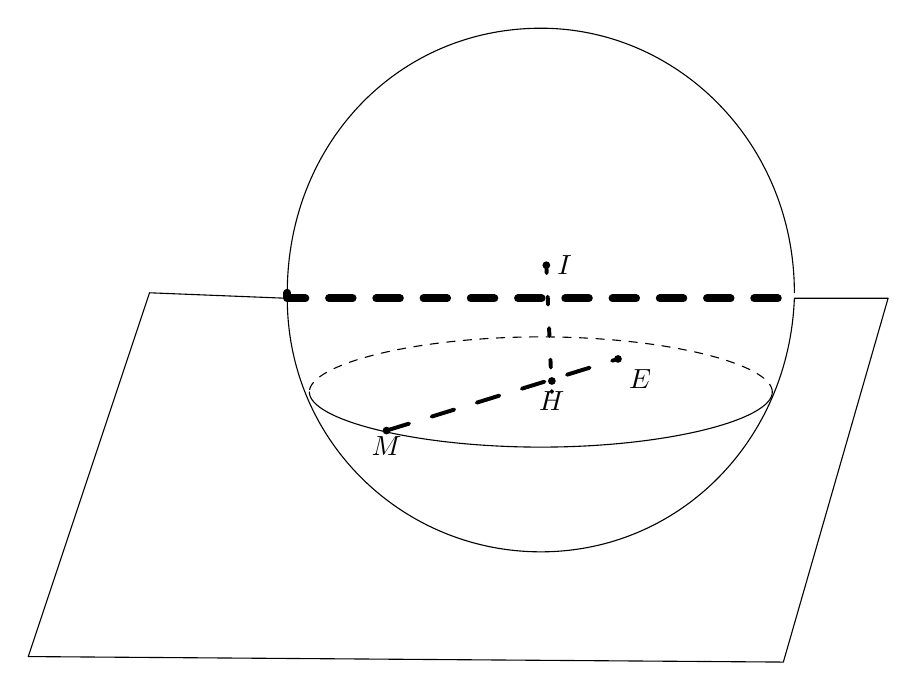
\begin{tikzpicture}[scale=.7,ethicknode/.append style={scale=1},line cap=round,line join=round,inner sep=0pt,outer sep=0pt]
		\draw 
			(17.5,12.1).. controls (17.4,9.5)  and (15.4,7.5).. (12.9,7.5)
			.. controls (10.4,7.5) and  (8.3,9.5).. (8.3,12.1) --
			 (5.8,12.2) -- (3.6,5.6) -- (17.3,5.5) -- (19.2,12.1) -- cycle;
		\draw 
			 (17.5,12.2).. controls (17.5,14.9) and (15.4,17.0).. (12.9,17.0)
			 .. controls (10.3,17.0) and (8.3,14.9).. (8.3,12.2);
		\draw[line width=1mm,dash pattern=on 3mm off 3mm] 
			(8.3,12.2) -- (8.3,12.1) -- (17.5,12.1) -- (17.5,12.2); 
		\draw[dashed] 
			 (17.1,10.4).. controls (17.1,10.9) and (15.2,11.4).. (12.9,11.4)
			 .. controls (10.6,11.4) and (8.7,10.9).. (8.7,10.4);
		 \draw
			(8.7,10.4)..  controls (8.7,9.9) and (10.6,9.4).. (12.9,9.4)
			.. controls (15.2,9.4)  and (17.1,9.9).. (17.1,10.4);
		\draw[line  width=.5mm,dash pattern=on 1mm off 3mm]
			(13.0,12.7)  -- (13.1,10.4);
		\fill (10.1,9.7) circle  (2pt) node[below=2pt]{$M$};
		\fill (13.1,10.6) circle (2pt)  node[below=4pt]{$H$};
		\fill  (14.3,11.0) circle (2pt) node[below right=4pt]{$E$};
		\fill (13.0,12.7) circle  (2pt) node[right=4pt]{$I$};
		\draw[line width=.5mm,dash pattern=on 3mm off 3mm] 
			 (10.1,9.7) -- (14.3,11.0);
	\end{tikzpicture}
\end{center}
Gọi $M(x;y;z)$. 
\begin{itemize}
	\item  Tập hợp điểm $M$ thỏa mãn $MA = \sqrt{2} MB$.
	\begin{eqnarray*}
		&& \sqrt{(x - 1)^2 + (y  - 1)^2 + (z - 2)^2} = \sqrt{2} \cdot \sqrt{(x + 1)^2 + (y - 2)^2 + (z - 1)^2} \\
		&\Rightarrow& (x - 1)^2 + (y - 1)^2 + (z - 2)^2 = 2\left[(x + 1)^2 +  (y - 2)^2 + (z - 1)^2\right] \\
		&\Rightarrow& x^2 + y^2 + z^2 +  6x - 6y + 6 = 0.
	\end{eqnarray*}
	Phương trình mặt cầu  tâm $I(-3; 3; 0)$, bán kính $R = 2\sqrt{3}$.
	\item Gọi $H$ là hình chiếu vuông góc của  $I$ lên $(P)$. \\
	Phương trình đường thẳng $d$ đi  qua $I$ và vuông góc với $(P)$ là $\heva{&x=-3+t\\&y=3+t,\, t\in\mathbb{R}\\&z=t.}$\\
	Xét  phương trình $(-3+t)+(3+t)+t-1=0\Leftrightarrow t=\dfrac{1}{3}$.\\
	Vậy $H\left(\dfrac{-8}{3};\dfrac{10}{3};\dfrac{1}{3}\right)$. 
	 \item Giao của mặt cầu với mặt phẳng $(P)$ với ($r$ là bán kính).
	\begin{eqnarray*}
		&& \mathrm{d}(I,(P)) = \dfrac{|-3 + 3 + 0 - 1|}{\sqrt{1^2 + 1^2 + 1^2}} = \dfrac{\sqrt{3}}{3}  \\
		&& r = \sqrt{R^2  - d^2} = \dfrac{\sqrt{105}}{3}.
	\end{eqnarray*}
	\item Giá trị lớn nhất của $EM$. Dễ  thấy điểm $E\in (P)$ và
	\begin{eqnarray*}
		&& EH =  \dfrac{\sqrt{6}}{3} \\
		&& EM_{\text{ max}} = HE  + r =\dfrac{\sqrt{6}}{3}+\dfrac{\sqrt{105}}{3}\approx 4{,}2.
	\end{eqnarray*}
\end{itemize}
Vậy giá  trị lớn nhất của $EM$ là $4{,}2$.
} 
\end{bt}

% nguồn: Phan2_Lop_12_Hinh_hoc_Chuong_5
\begin{bt}%[2H5V3-3]%[ma:fccbc321]
	Cho $3$ điểm $M(2;3;3)$, $N(2;-1;-1)$, $P(-2;-1;3)$ và mặt  phẳng $(\alpha)\colon 2x+3y-z+2=0$. Phương trình mặt cầu đi qua $3$ điểm $M$, $N$, $P$ và có tâm thuộc mặt phẳng $(\alpha)$ có bán kính bằng bao nhiêu?
	\shortans{4} 
	 \loigiai{
		Phương trình  mặt cầu $(S)$ có dạng $x^2+y^2+z^2-2ax-2by-2cz+d=0$ với
		 $a^2+b^2+c^2-d>0$.\\
		Mặt cầu qua $M$, $N$, $P$, suy ra $\heva{& 4a+6b+6c-d=22  \\&4a-2b-2c-d=6\\& 4a+2b-6c+d=-14.}$\\
		Mặt cầu có tâm $I(a;b;c)$ thuộc mặt  phẳng $(\alpha)\Rightarrow 2a+3b-c+2=0$.\\
		Giải hệ ta được $\heva{& a=2\\& b=-1\\& c=3\\&  d=-2}\Rightarrow I(2;-1;3)$.\\
		Bán kính của mặt  cầu là $R=\sqrt{a^2+b^2+c^2-d}=\sqrt{2^2+(-1)^2+3^2-(-2)}=4$.
	} 
\end{bt}

% nguồn: Phan2_Lop_12_Hinh_hoc_Chuong_5
\begin{bt}%[2H5C3-3]%[ma:d5175057]
	Trong không gian với hệ tọa độ Oxyz cho ba điểm $A(8;5;-11)$, $B(5;3;-4)$, $C(1;2;-6)$ và mặt cầu $(S)\colon (x-2)^2 + (y-4)^2 + (z+1)^2 = 9$. Gọi $M(a;b;c)$ là điểm thuộc mặt cầu $(S)$ sao cho $|\overrightarrow{MA} - \overrightarrow{MB} -  \overrightarrow{MC}|$ đạt giá trị nhỏ nhất. Tính giá trị biểu thức $T = a+b+c$.
	\shortans{2} 
	\loigiai{ 
		Gọi $I(x,y,z)$ là điểm thỏa mãn $\overrightarrow{IA} - \overrightarrow{IB} - \overrightarrow{IC}  = \overrightarrow{0}$. Khi đó $I(-2; 0; 1)$.
		 Ta có
		\allowdisplaybreaks 
		\begin{eqnarray*}
			\left| \overrightarrow{MA} - \overrightarrow{MB} - \overrightarrow{MC} \right| &=& \left| (\overrightarrow{MI} + \overrightarrow{IA}) - (\overrightarrow{MI} + \overrightarrow{IB}) - (\overrightarrow{MI}  + \overrightarrow{IC})\right| \\
			&=& \left| \overrightarrow{MI} + \overrightarrow{IA} - \overrightarrow{MI} - \overrightarrow{IB} -  \overrightarrow{MI} - \overrightarrow{IC} \right|\\
			&=& \left|  (\overrightarrow{IA} - \overrightarrow{IB} - \overrightarrow{IC}) - \overrightarrow{MI}\right|\\
			&=&  \left| - \overrightarrow{MI}\right| = MI.
		\end{eqnarray*}
		Mặt cầu $(S)$ có tâm là $K(2; 4;  -1)$ và bán kính $R = 3$.\\
		Để $|\overrightarrow{MA} - \overrightarrow{MB} - \overrightarrow{MC}|$ đạt giá trị nhỏ  nhất thì $MI$ phải nhỏ nhất $\Leftrightarrow M=KI\cap (S)$.\\
		Ta có $\overrightarrow{KI} = (-4; -4; 2)$. Chọn $\vec{u} = (-2;-2;1)$  là VTCP của $KI$.\\
		Phương trình tham số của $KI$ là $ \heva{&x = 2 - 2t \\ &y  = 4 - 2t \\ &z = -1 + t.} $\\
		Vì  $M=KI\cap (S)$ nên tọa độ $M$ được xác định bởi phương trình
		\[\left[(2-2t)-2 \right]^2  + \left[(4-2t)-4\right]^2 + \left[(-1+t)+1\right]^2 = 9 \Leftrightarrow \hoac{&t=1 \\& t= -1.} \]
		Với $t=1$ thì $x = 0$, $y = 2$, $z = 0$. Suy ra $M_1(0; 2; 0)$ và  $M_1I = 3$.\\
		Với $t=-1$ thì  $x = 4$, $y = 6$, $z = -2$. Suy ra $M_2(4; 6; -2)$ và $M_2I = 9$.\\
		Do $M_1I < M_2I$ nên điểm $M_1 (0;2;0)$ thỏa mãn yêu  cầu đề bài.\\
		Suy ra $T = a+b+c = 0+2+0  = 2$.
	 }
\end{bt}

% nguồn: Phan2_Lop_12_Hinh_hoc_Chuong_5
\begin{bt}%[2H5C3-3]%[ma:169cdb11]
	Trong không gian $Oxyz$, cho ba điểm $A(0; 3;-5)$, $B(1; 1;-5)$, $C(4; 3;-1)$ và mặt cầu $(S)\colon x^2+y^2+z^2+(m-2)x+4y+(m-2)z-3=0$ ($m$ là tham số thực). Gọi $(T)$ là tập hợp tất cả điểm cố định mà mặt cầu $(S_m)$ luôn đi qua với mọi số thực $m$ và $M$ là một điểm di động trên $(T)$ sao cho thể tích tứ  diện $MABC$ đạt giá trị lớn nhất. Tính giá trị lớn nhất đó (làm tròn đến hàng phần chục).
	\shortans{15,3} 
	 \loigiai{
		Xét $M(x; y; z)$ là điểm  mà $(S_m)$ luôn đi qua với mọi $m$. \\
		Ta có 
		\begin{eqnarray*}
			&&  x^2+y^2+z^2+(m-2)x+4y+(m-2)z-3=0, \forall m\in \mathbb{R} \\
			&\Leftrightarrow&  m(x+z)+x^2+y^2+z^2-2x+4y-2z-3=0, \forall m\in \mathbb{R} \\
			&\Leftrightarrow& \heva{& x+z=0\\&x^2+y^2+z^2-2x+4y-2z-3=0.} 
		\end{eqnarray*}
		Tập hợp  các điểm $M$ cần tìm là đường tròn $(C)$, trong đó $(C)$ là giao tuyến của mặt phẳng $(P)\colon x+z=0$ và mặt cầu có tâm $I(1;-2; 1)$, bán kính $R=3$.
		 \[\mathrm{d}\left(I,(P)\right)=\dfrac{\left|1+1\right|}{\sqrt{2}}=\sqrt{2}.\]
		Vì vậy $(C)$ có bán  kính là $r=\sqrt{R^2-d^2\left(I, (P)\right)}=\sqrt{7}$ và tâm $J(0;-2; 0)$. \\
		 Mặt phẳng $(ABC)$ có phương trình $2x+y-2z-13=0$. \\
		Ta thấy $(ABC)$ vuông góc với $(P)$.  \\
		Ta có $\heva{&\overrightarrow{AB}=(1;-2; 0)  \\&\overrightarrow{AC}=(4; 0; 4)} \Rightarrow \left[\overrightarrow{AB},\overrightarrow{AC}\right]=(-8;-4; 8) \Rightarrow S_{ABC}=\dfrac{1}{2} \cdot \sqrt{64+16+64}=6$. \\
		Thể tích  tứ diện $MABC$ là
		\[V_{MABC}=\dfrac{1}{3} \mathrm{d}\left(M, (ABC)\right)\cdot S_{ABC}=2 \mathrm{d}\left(M, (ABC)\right).\] 
		Thể tích này lớn nhất khi và chỉ khi $\mathrm{d}\left(M, (ABC)\right)$  đạt giá trị lớn nhất. \\
		 Ta có
		\begin{eqnarray*}
			\mathrm{d}\left(M, (ABC)\right)_{\max}&=&r+\mathrm{d}\left(J, (ABC)\right) \\ 
			&=&\sqrt{7}+\dfrac{\left|2 \cdot 0-2-2 \cdot 0-13\right|}{\sqrt{2^2 +1^2 +  (-2)^2}}=\sqrt{7}+5.
		\end{eqnarray*}
		 Vì vậy $V_{\max}=2\sqrt{7}+10\approx 15{,}3$.
	 }
\end{bt}


%%%%%%%%%%%%%%%% TỰ LUẬN %%%%%%%%%%%%%%%%

% nguồn: Phan2_Lop_12_Hinh_hoc_Chuong_5
\begin{bt}%[2H5H3-3]%[ma:cc9bc3f4]
	Trong không gian $Oxyz$, cho điểm $I\left(1;-2;3\right)$. Viết phương trình mặt cầu tâm $I$, cắt trục $Ox$ tại hai điểm $A$ và $B$ sao cho  $AB=2\sqrt 3 $.
	\loigiai{ 
		Gọi $H$ là trung điểm của $AB$ thì $IH$ vuông góc với $AB$ và  $IH=\sqrt{\left(-2\right)^2+3^2}=\sqrt{13}$.\\
		 Suy ra bán kính mặt cầu là $R=IA=\sqrt{3+13}=4$.\\
		Vậy phương trình  mặt cầu là $$\left(x-1\right)^2+\left(y+2\right)^2+\left(z-3\right)^2=16.$$
	} 
\end{bt}

% nguồn: Phan2_Lop_12_Hinh_hoc_Chuong_5
\begin{bt}%[2H5H3-3]%[ma:9a4b871d]
	Trong không gian $Oxyz$, gọi $(P)$ là mặt phẳng đi qua  điểm $A\left(1;4;-3\right)$ và chứa trục $Ox$. Viết phương trình mặt cầu $(S)$ có tâm $I\left(1;2;1\right)$ và tiếp xúc với mặt phẳng $(P)$.
	\loigiai{ 
		Ta có $\overrightarrow{OA}=\left(1;4;-3\right)$ nên $\left[\overrightarrow{OA},\overrightarrow i\right]=\left(0;-3;-4\right)$ khi đó mặt phẳng $(P)$ đi qua điểm $A\left(1;4;-3\right)$ và có véctơ pháp tuyến $\overrightarrow n=\left(0;3;4\right)$  nên phương trình mặt phẳng $(P)$ là $3y+4z=0$.\\
		Lại có  $\mathrm{d}\left(I,(P)\right)=\dfrac{\left|3\cdot 2+4\cdot 1\right|}{\sqrt{3^2+4^2}}=2$.\\
		Mặt  cầu tâm $I\left(1;2;1\right)$ bán kính $R=\mathrm{d}\left(I,(P)\right)=2$ có phương trình là
		 $$\left(x-1\right)^2+\left(y-2\right)^2+\left(z-1\right)^2=4.$$
	 }
\end{bt}

% nguồn: Phan2_Lop_12_Hinh_hoc_Chuong_5
\begin{bt}%[2H5H3-3]%[ma:ceb69d8d]
	 Trong không gian với hệ trục tọa độ $Oxyz$, hãy viết phương trình mặt cầu đi qua $ 3 $ điểm $A\left(-2;3;3\right)$, $B\left(-1;1;2\right)$, $C\left(4;2;2\right)$ và có tâm nằm thuộc mặt phẳng $\left(Oyz\right)$.
	\loigiai{ 
		Vì mặt cầu  có tâm $I$ thuộc mặt phẳng $\left(Oyz\right)$ nên tâm có dạng $I\left(0;b;c\right)$.\\
		 Vì mặt cầu đi qua ba điểm $A\left(-2;3;3\right)$, $B\left(-1;1;2\right)$, $C\left(4;2;2\right)$ nên ta có
		\begin{eqnarray*}
			&IA=IB=IC=R&\Leftrightarrow IA^2=IB^2=IC^2=R^2\\ 
			& &\Leftrightarrow\heva{& 
			 4+\left(3-b\right)^2+\left(3-c\right)^2=1+\left(1-b\right)^2+\left(2-c\right)^2\\
			 &1+\left(1-b\right)^2+\left(2-c\right)^2=16+\left(2-b\right)^2+\left(2-c\right)^2
			}\\ 
			& &\Leftrightarrow\heva{& 
			40+9-6c+c^2=65+4-4c+c^2\\ 
			 &b=9
			}\\ 
			& &\Leftrightarrow\heva{& 
			 -2c=20\\
			&  b=9
			}\Leftrightarrow\heva{ 
			&  c=-10\\
			 & b=9.
			 }
		\end{eqnarray*}
		Suy ra  $ I\left(0;9;-10\right)$, $R=IA=\sqrt{4+36+169}=\sqrt{209}$.\\
	Phương trình mặt  cầu là $x^2+\left(y-9\right)^2+\left(z+10\right)^2=209$}
\end{bt}

% nguồn: Phan2_Lop_12_Hinh_hoc_Chuong_5
\begin{bt}%[2H5H3-3]%[ma:7af61e20]
	Cho hình hộp chữ nhật $OABC.O'A'B'C'$,  với $O$ là gốc toạ độ, $A(2;0;0)$, $C(0; 6; 0)$, $O'(0; 0; 4)$. Viết phương trình
	\begin{enumerate}
		\item mặt phẳng $\left(O'A  C\right)$;
		\item  đường thẳng $CO'$;
		 \item mặt cầu đi qua các đỉnh của hình hộp.
	\end{enumerate}
	 \loigiai{
		\begin{enumerate}
			\item Ta có $\overrightarrow{O'A}=\left(2; 0; -4\right)$,  $\overrightarrow{O'C}=\left(0; 6; -4\right)$.\\
			Mặt phẳng $(O' A C)$ đi  qua $A\left(2; 0; 0\right)$ và nhận $\left[\overrightarrow{O' A},\overrightarrow{O' C} \right]=\left(-24; 8; 12\right)$ làm vectơ pháp tuyến. Phương trình $\left(O' A C\right)$ là $$-24\left(x-2\right)+8\left(y-0\right)+12\left(z-0\right)=0\Leftrightarrow -6x+2y+3z+12=0.$$
			\item Đường thẳng $C O'$ đi qua  điểm $C\left(0; 6; 0\right)$ và nhận $\overrightarrow{CO'}=\left(0; -6; 4\right)$ làm vectơ chỉ phương. Phương trình tham số của đường thẳng $CO'$ là $\heva{&x=0\\&y=6-6t\\&z=4t}$.
			\item Vì hình hộp chữ nhật $O A B C.O'A'B'C'$, với $O$ là gốc toạ độ, $A(2; 0; 0), C(0; 6; 0)$, $O'(0; 0;  4)$ nên $B'\left(2; 6; 4\right)$.\\
			Ta có $OB'=3\sqrt{6}$ là đường kính của  mặt cầu ngoại tiếp hình hộp chữ nhật nên\break $R=\dfrac{OB'}{2}=\dfrac{3\sqrt{6}}{2}$. Gọi $I$ là tâm mặt cầu ta có $I\left(1; 3; 2\right)$.\\
			Mặt cầu đi qua các đỉnh của hình  hộp chữ nhật có phương trình là $$\left(x-1\right)^2+\left(y-3\right)^2+\left(z-2\right)^2=\dfrac{27}{2}.$$
		\end{enumerate}
	 }
\end{bt}

% nguồn: Phan2_Lop_12_Hinh_hoc_Chuong_5
\begin{bt}%[2H5H3-3]%[ma:db887513]
	Viết  phương trình mặt cầu $(S)$
	\begin{enumerate}
		 \item có tâm $I\left(7;-3;0\right)$, bán kính $R=8$.
		\item có tâm $M\left(3;1;-4\right)$ và đi qua điểm  $N\left(1;0;1\right)$.
		\item có đường  kính $AB$ với $A\left(4;6;8\right)$ và $B\left(2;4;4\right)$.
	\end{enumerate}
	\loigiai{ 
		\begin{enumerate}
			\item Phương trình mặt cầu $(S)$ có  tâm $I\left(7;-3;0\right)$, bán kính $R=8$ là\\
			 $\left(x-7\right)^2+\left(y+3\right)^2+z^2=8^2$ hay $\left(x-7\right)^2+\left(y+3\right)^2+z^2=64$.
			\item Mặt cầu $(S)$ có  tâm $M\left(3;1;-4\right)$ và đi qua điểm $N\left(1;0;1\right)$ nên có bán kính $R=MN=\sqrt{30}$.\\
			Vậy mặt cầu $(S)$ có phương  trình là $$\left(x-3\right)^2+\left(y-1\right)^2+\left(z+4\right)^2=30.$$
			\item Mặt cầu $(S)$ có đường kính $AB$ với $A\left(4;6;8\right)$ và $B\left(2;4;4\right)$ nên có tâm $J\left(3;5;6\right)$ là trung điểm của $AB$ và bán kính $R=AJ=\sqrt  6 $.\\
			Vậy mặt cầu $(S)$ có phương trình  là $$\left(x-3\right)^2+\left(y-5\right)^2+\left(z-6\right)^2=6.$$
		\end{enumerate}
	} 
\end{bt}

% nguồn: Phan2_Lop_12_Hinh_hoc_Chuong_5
\begin{bt}%[2H5H3-3]%[ma:8a75b23a]
	Trong không gian $Oxyz$,  lập phương trình của mặt cầu $(S)$ biết mặt cầu $(S)$ có đường kính $AB$ với $A(3;2;-1)$ và $B(-1;2;2)$.
	 \loigiai{
		Đoạn thẳng $AB$ có trung điểm  $I\left( 1;2;\dfrac{1}{2}\right) $.\\
		Mặt  cầu $(S)$ có tâm $I$ và bán kính $R=\dfrac{1}{2}AB=\dfrac{1}{2}\sqrt{(-1-3)^2+(2-2)^2+(2+1)^2}=\dfrac{5}{2}$.\\
		Phương  trình của $(S)$ là $(x-1)^2+(y-2)^2+(z-\dfrac{1}{2})^2=\dfrac{25}{4}$.
	 }
\end{bt}

% nguồn: Phan2_Lop_12_Hinh_hoc_Chuong_5
\begin{bt}%[2H5H3-3]%[ma:94261ccd]
	Trong không gian $Oxyz$, viết phương  trình mặt cầu $(S)$ có tâm $A\left(1;2;-3\right)$ và tiếp xúc với trục $Ox$.
	 \loigiai{
		Ta có $R=\mathrm{d}\left(A,Ox\right)=\sqrt{2^2+\left(-3\right)^2}=\sqrt{13}$.\\ 
		Phương trình mặt cầu $(S)$ có tâm $A\left(1;2;-3\right)$, bán kính $R=\sqrt{13}$ có phương trình  là
	$$(S)  \colon \left(x-1\right)^2+\left(y-2\right)^2+\left(z+3\right)^2=13.$$}
\end{bt}

% nguồn: Phan2_Lop_12_Hinh_hoc_Chuong_5
\begin{bt}%[2H5H3-3]%[ma:17a55686]
	Trong không gian $Oxyz$, cho điểm $A\left(1;-1;1\right)$ và đường thẳng. Gọi $(P)$ là mặt phẳng đi qua $A$ và chứa $d$. Lập phương trình mặt cầu  $(S)$ có tâm $I\left(2;3;-1\right)$ sao cho tiếp xúc với $(P)$.
	\loigiai{ 
		Đường thẳng $d$ đi qua  $M\left(0;-1;2\right)$ và có vectơ chỉ phương $\overrightarrow u=\left(1;-2;-2\right)$.\\
		Mặt phẳng $(P)$ có vectơ pháp tuyến  $\overrightarrow n=\left[\overrightarrow{AM};\overrightarrow u\right]=\left(2;-1;2\right)\Rightarrow(P)\colon 2x-y+2z-5=0$.\\
	Bán kính mặt cầu $R=\mathrm{d}\left(I;(P)\right)=2$ nên phương trình mặt cầu là  $$\left(x-2\right)^2+\left(y-3\right)^2+\left(z+1\right)^2=4.$$}
\end{bt}

% nguồn: Phan2_Lop_12_Hinh_hoc_Chuong_5
\begin{bt}%[2H5H3-3]%[ma:9e0dcaf5]
	Trong không gian với hệ trục tọa độ $Oxyz$, cho điểm $A\left(-2;-4;5\right)$.  Viết phương trình của mặt cầu tâm là $A$ và cắt trục $Oz$ tại hai điểm $B$, $C$ sao cho $\Delta ABC$ vuông.
	 \loigiai{
		Do $AB=AC$ nên $\Delta ABC$ vuông tại $A$. Gọi  $H$ trung điểm $BC$ suy ra $AH=BH=HC$.\\
		Do đó $H$ là hình chiếu của điểm $A$  lên trục $Oz$.\\
		 ta có $A{B^2}=A{H^2}+B{H^2}=2A{H^2}$.\\
		Suy ra $R=AH\sqrt 2 =\mathrm{d}\left(A,Oz\right)\cdot  \sqrt 2 =\sqrt{x_A^2+y_A^2}\cdot \sqrt 2 =2\sqrt{10}$.\\
		Vậy mặt cầu có phương  trình $$\left(x+2\right)^2+\left(y+4\right)^2+\left(z-5\right)^2=40.$$
	} 
\end{bt}

% nguồn: Phan2_Lop_12_Hinh_hoc_Chuong_5
\begin{bt}%[2H5H3-3]%[ma:e732eb71]
	Trong không gian $Oxyz$, viết phương trình mặt cầu có tâm nằm trên mặt phẳng $\left(Oyz\right)$ và đi qua các điểm $A\left(0;8;0\right)$, $B\left(4;6;2\right)$,  $C\left(0;12;4\right)$.
	\loigiai{ 
		Gọi  tâm mặt cầu là $I\left(0;b;c\right)\in\left(Oyz\right)$.\\
		Do  $A\left(0;8;0\right)$, $B\left(4;6;2\right)$, $C\left(0;12;4\right)$ thuộc mặt cầu nên\\
		Khi  đó
		\begin{eqnarray*}
			 &IA=IB=IC&\Leftrightarrow{\left(b-8\right)^2}+c^2=16+\left(b-6\right)^2+\left(c-2\right)^2=\left(b-12\right)^2+\left(c-4\right)^2\\
			&  &\Leftrightarrow\heva{&{b-c=2}\\&{b+c=12}}\Leftrightarrow\heva{&{b=7}\\& {c=5}}
		\end{eqnarray*}
		Vậy $I\left(0;7;5\right)$;  $R=IA=\sqrt{26}$.\\
	Phương trình  mặt cầu là $x^2+\left(y-7\right)^2+\left(z-5\right)^2=26$}
\end{bt}

% nguồn: Phan2_Lop_12_Hinh_hoc_Chuong_5
\begin{bt}%[2H5H3-3]%[ma:0e4b05e8]
	Trong không gian với hệ tọa độ $Oxyz$, cho các điểm $A\left(6;0;0\right)$, $B\left(0;4;0\right)$ và $C\left(0;0;2\right)$. Viết phương trình  mặt cầu ngoại tiếp tứ diện $OABC$.
	 \loigiai{
		Phương  trình mặt cầu ngoại tiếp tứ diện $OABC$ có dạng
		$$x^2+y^2+z^2-2ax-2by-2cz+d=0\,\left(a^2+b^2+c^2-d >  0\right).$$
		 Do $O$, $A$, $B$, $C\in(S)\Rightarrow\heva{&d=0\\&36-12a+d=0\\& 16-8b+d=0\\&4-4c+d=0
		}\Leftrightarrow\heva{& d=0\\& a=3\\& b=2\\&  c=1}\Rightarrow R=\sqrt{a^2+b^2+c^2-d}=\sqrt{14}$.\\
	Mặt cầu tâm  $I\left(3;2;1\right)$, $R=\sqrt{14}$ có phương trình $$\left(x-3\right)^2+\left(y-2\right)^2+\left(z-1\right)^2=14.$$}
\end{bt}
